\documentclass[a4paper,10pt]{article}
\usepackage{latexsym}
\usepackage{amsmath}
\usepackage{amssymb}
\usepackage{bm}
\usepackage{graphicx}
\usepackage{wrapfig}
\usepackage{fancybox}
\pagestyle{plain}

\begin{document}

Flow Guided Recurrent Neural Encoder for Video Salient Object Detection

Guanbin $\mathrm{L}\mathrm{i}^{1}$ Yuan Xiel Tianhao Wei2 Keze Wangl Liang $\mathrm{L}\mathrm{i}\mathrm{n}^{1,3*}$

lSun $\mathrm{Y}\mathrm{a}\mathrm{t}.-\mathrm{s}\mathrm{e}\mathrm{n}\mathrm{U}\mathrm{n}\mathrm{i}\mathrm{v}\mathrm{e}\mathrm{r}\mathrm{s}\mathrm{i}\mathrm{t}\mathrm{y}^{2}$Zhejiang University.$3$SenseTime.Group L$\mathrm{i}\mathrm{m}\mathrm{i}\mathrm{t}\mathrm{e}\mathrm{d}1_{9^{\mathrm{U}i}},\mathrm{n}\mathrm{b}\mathrm{i}\mathrm{n}\otimes i,$

wangkeze\S mai12. sysu. edu. cn, linliang\S ieee. org

Abstract

{\it Image saliency detection has recently witnessed signif}- {\it icant progress due to deep convolutional neural networks. However extending state-of-the-art saliency detectors from image to video is challenging. The perormance of salient object detection suers from object or camera motion and the dramatic change of the appearance contrast in videos. In this paper we present flow guided recurrent neural encoder} ({\it FGRNE}), {\it an accurate and end-to-end learning framework for video salient object detection. It works by enhancing the temporal coherence of the per-frame feature by exploiting both motion information in terms of optical flow and sequential feature evolution encoding in terms of LSTM networks. It can be considered as a universal frame}- {\it work to extend any} $FCN$ {\it based static saliency detector to video salient object detection. Intensive experimental re}- {\it sults veri the eectiveness of each part of FGRNE and confirm that our proposed method significantly outperorms state-of-the-art methods on the public benchmarks ofDAVIS}

{\it and FBMS}.
\begin{center}
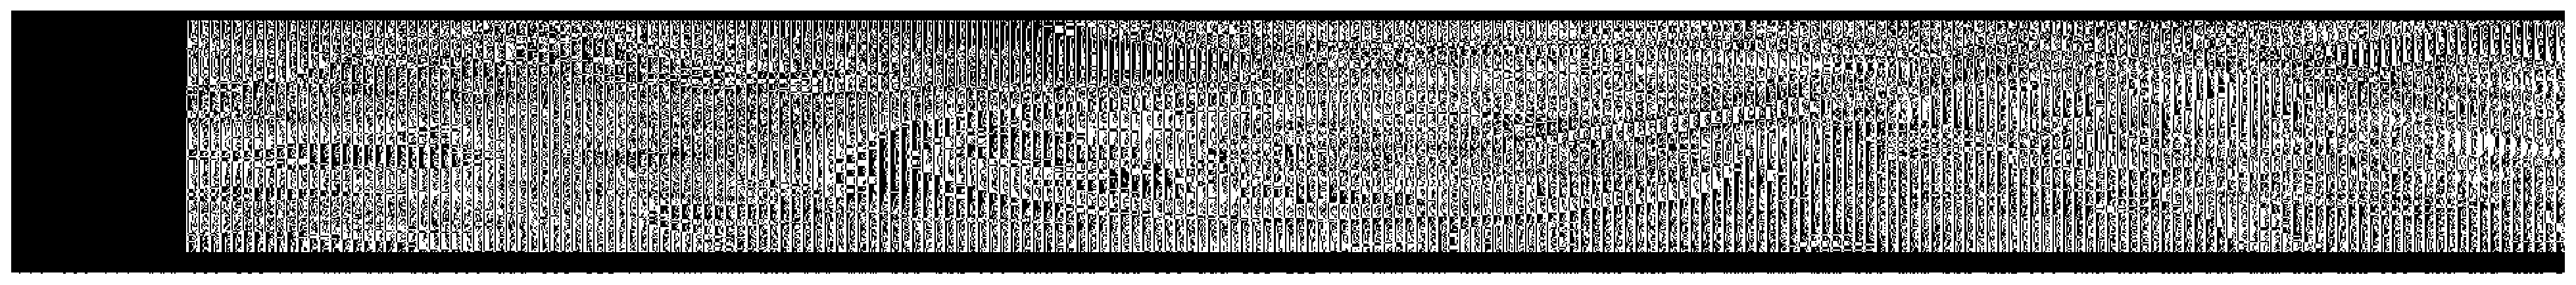
\includegraphics[width=78.91mm,height=8.13mm]{./CVPR2018_VideoSaliency_images/image001.eps.eps}

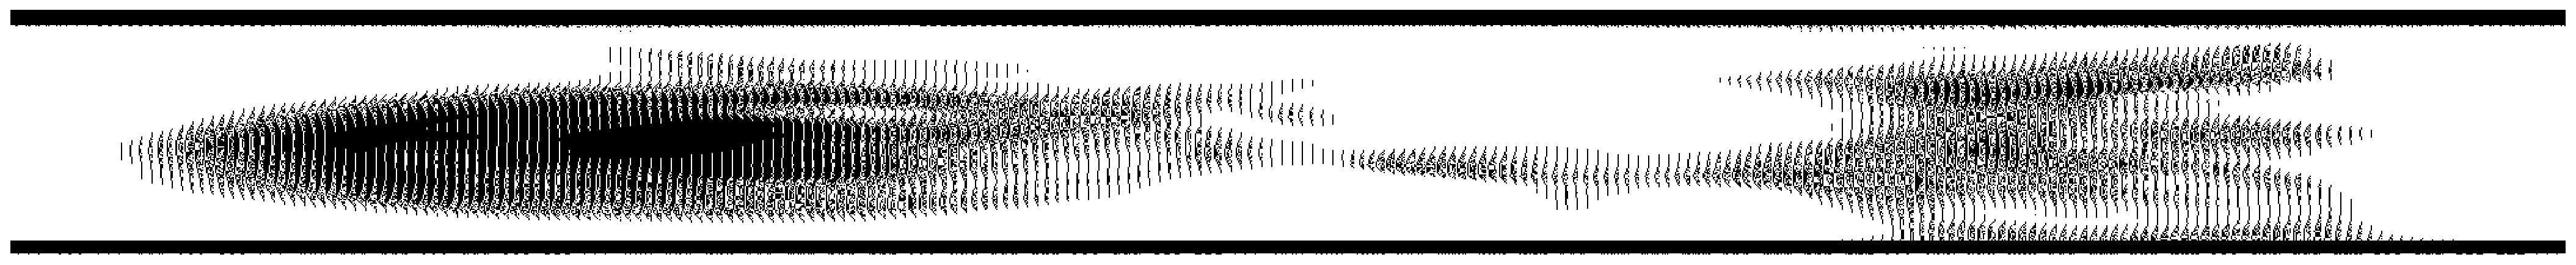
\includegraphics[width=85.01mm,height=8.13mm]{./CVPR2018_VideoSaliency_images/image002.eps.eps}

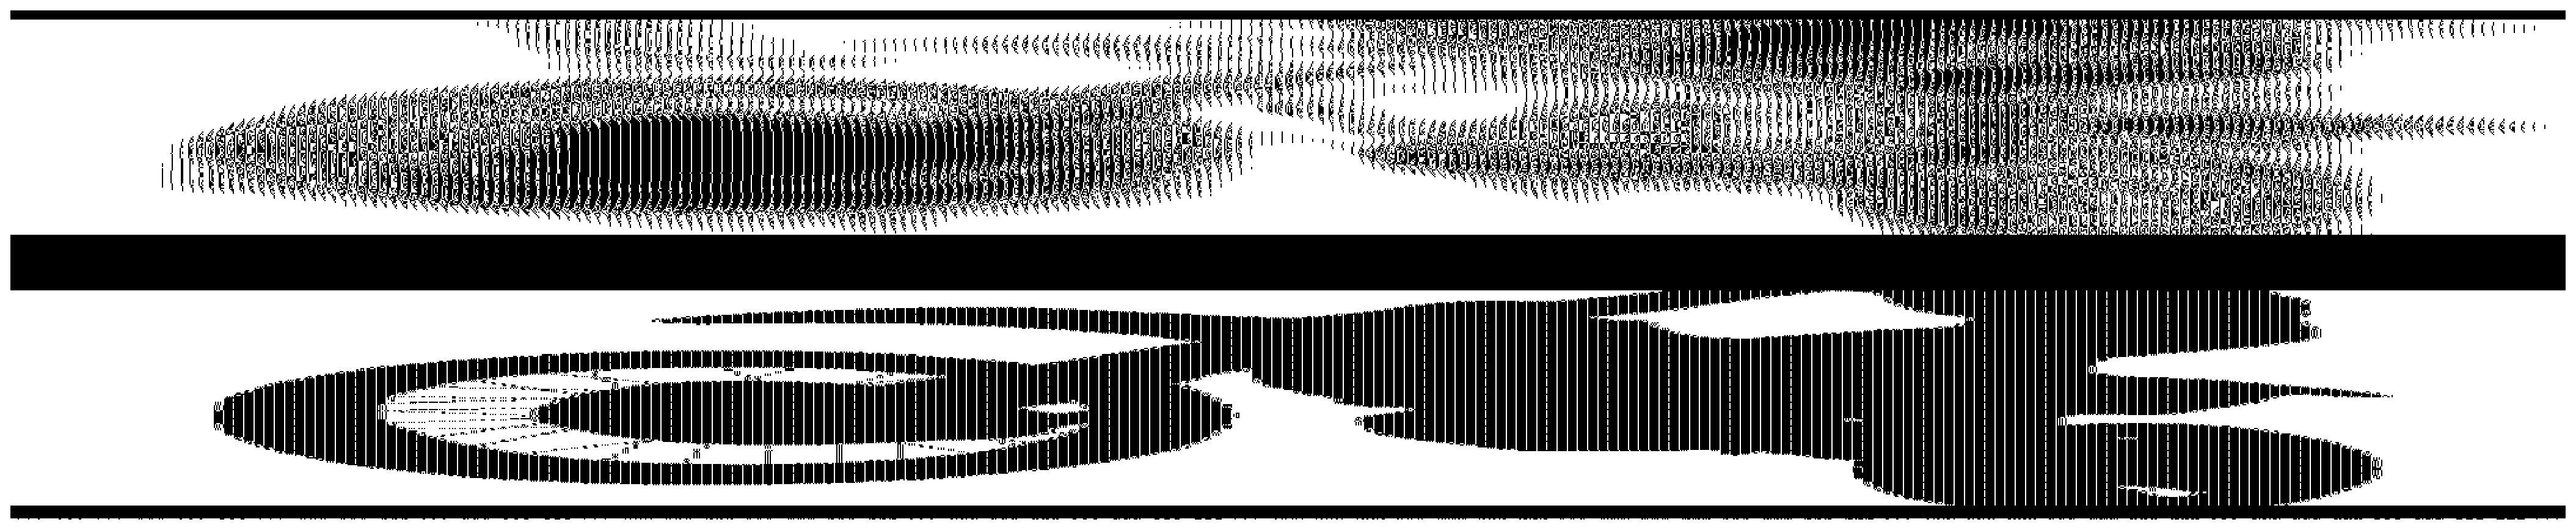
\includegraphics[width=85.01mm,height=16.93mm]{./CVPR2018_VideoSaliency_images/image003.eps.eps}
\end{center}
1. Introduction

Salient object detection aims at identifying the most vi- sually distinctive objects in an image or video that attract human attention. It has drawn a lot of attention due to the need for solving this problem in many computer vision ap- plications such as image and video compression [{\it 12}], ob- ject segmentation $[^{\fbox{$\mathrm{Error}::0\mathrm{x}0000$}}3_{7^{7}}^{\prime^{-}}$], visual tracking $[^{\fbox{$\mathrm{Error}::0\mathrm{x}0000$}}3_{\ovalbox{\tt\small REJECT}}8_{\ovalbox{\tt\small REJECT}}$] and person re- identification $[4^{\fbox{$\mathrm{Error}::0\mathrm{x}0000$}}3]$. Although image based salient object de- tection has been extensively studied during the past decade, video based salient object detection is much less explored

$*$The first two authors contribute equally to this paper. Correspond- ing author is Liang Lin. This work was supported by the State Key Development Program under Grant $2016\mathrm{Y}\mathrm{F}\mathrm{B}1001004$, the National Nat- ural Science Foundation of China under Grant 61702565, Guangdong Natural Science Foundation Project for Research Teams under Grant $2017\mathrm{A}030312006$, and was also sponsored by CCF-Tencent Open Re- search Fund.

due to its high complexity and the lack of large-scale anno- tated video datasets.

GT

Figure 1. The challenges of still-image saliency detector and the effectiveness of temporal coherence modeling in video based salient object detection.

In recent years, due to the success deployment of deep convolutional neural networks (CNN), the performance of salient object detection in static image has been increased by a significant margin $[$21., 1 1 $24_{-}0]$. Nevertheless, di- rectly applying these methods to video salient object de- tection is non-trivial and challenging. The performance of salient object detection suffers from object or camera mo- tion and the dramatic change of the appearance contrast in videos. As shown in the second row of Fig. 1, state-of- the-art still-image salient object detectors (e.g. DSS $[1.4_{-}0]$) deteriorates drastically from the inability to maintain the vi- sual continuity and temporal correlation of salient objects between consecutive frames.

Cognitive studies have shown that visual contrast is the key factor that leads to a specific region becoming salient in static images. For dynamic videos, the difference be- tween consecutive frames caused by object motion are more attractive to people's attention $[1..\fbox{$\mathrm{Error}::0\mathrm{x}0000$}3]$. Such tempo- ral information has been exploited in existing video salient object detection methods either in the form of graphics model $[..3_{5}^{5}),\ ..3]$ or simply embedded in a convolutional neu- ral network $[^{\fbox{$\mathrm{Error}::0\mathrm{x}0000$}}36_{\backslash }6$]. Graphics model based methods generally employ generative framework which first infers an initial saliency map from either intra-frame appearance contrast

information $[^{\fbox{$\mathrm{Error}::0\mathrm{x}0000$}}3$] or inter-frame gradient flow field $[\cdots$�k$3_{\fbox{$\mathrm{Error}::0\mathrm{x}0000$}}^{5}55]$, and further incorporates an energy function with some heuris- tic spatio-temporal modeling to encourage the cross-frame consistency of the output saliency maps. Due to their in- dependence from training data and the use of handcrafted low-level features, it is arduous for graphics model based methods to cope with videos with complex semantic con- trast and objects motion. Although optical flow has been exploited in these methods, it is only used in an off-the- shelf mode for heuristic post-processing. Recently, with the thriving application of deep CNN in salient object de- tection of static images, there are also attempts to extend CNN to video salient object detection $[^{3}36,1$ They simply concatenate consecutive frame images and feed to convo- lutional neural networks for temporal coherence modeling. However, since convolutional neural network does not have the memory function, this naive aggregation of raw frame images followed by a serious of convolution operations can not well characterize the continuous dynamic evolution of video frames in the temporal domain. Moreover, this simple spatio-temporal modeling strategy lacks explicit compensa- tion for object's motion, making it hard to detect the salient objects with strenuous movement while maintaining tempo- ral coherence (e.g. object moves beyond the receptive field of the neural network).

In this work, we present flow guided recurrent neural en- coder (FGRNE), an end-to-end learning framework to ex- tend any FCN based still-image saliency detectors to video salient object detection. It works by enhancing the tempo- ral coherence of the per-frame feature by exploiting both motion information in terms of optical flow and sequen- tial feature evolution encoding in terms of LSTM networks. Specifically, we employ an off-the-shelf FCN based image saliency detector (e.g. DSS [10]) as our host network for feature extraction and ultimate saliency inference, and a pre-trained FlowNet [7] for motion estimation between a frame pair. Our FGRNE learns to improve the per-frame feature by incorporating a flow guided feature warping fol- lowed by a LSTM based temporal coherence feature encod- ing. The output feature map at the last time-step is con- sidered as our encoded feature and is fed to the upper part of the host network for saliency inference. Moreover, our FGRNE also involves another LSTM module to improve the estimated optical flow from frame pairs with large time interval. All the three modules of FGRNE including mo- tion computing and updating, flow guided feature warping as well as temporal coherence feature encoding are trained end-to-end with the host network.

In summary, this paper has the following contributions:

$\bullet$ We introduce a flow guided recurrent neural encoder framework to enhance the temporal coherence mod- eling of the per-frame feature representation, which can be exploited to extend any FCN based still-image

saliency detector to video salient object detection.

$\bullet$ We propose to incorporate an optical flow network in FGRNE framework to estimate the motion of each frame, which is further used in feature warping to ex- plicitly compensate for object's motion.

$\bullet$ We proposed to exploit a ConvLSTM in our FGRNE for sequential feature encoding, which can capture the evolution of appearance contrast in temporal domain and is complementary to feature warping towards an improved performance for video salient object detec- tion.

2. Related Work

2.1. StillImage Salient Object Detection

Image salient object detection has been extensively stud- ied for decades. Conventional methods can be divided into bottom-up approaches based on low-level features $[8_{\fbox{$\mathrm{Error}::0\mathrm{x}0000$}}.8,\ 1\ 5\backslash 555]$ and top-down models guided by high-level knowledge [1.4, $44_{-}0,2^{:}2]$. In recent years, the profound deep CNN has pushed the research on salient object detection into a new phase and has become the dominant research direction in this field. Deep CNN based methods can be further divided into two categories, including region based deep feature learn- ing $[1_{\nu}^{(:}\fbox{$\mathrm{Error}::0\mathrm{x}0000$}9,\ 42,\ ..\fbox{$\mathrm{Error}::0\mathrm{x}0000$}3^{:}2]$ and end-to-end fully convolutional network based methods $[24_{-}0,1$ 1 $\fbox{$\mathrm{Error}::0\mathrm{x}0000$}3^{\fbox{$\mathrm{Error}::0\mathrm{x}0000$}}3,1$ Methods in the first category separate an image into regions, and treat each re- gion as an independent unit for deep feature extraction and saliency inference. They are generally space and time con- suming due to significant redundancy in feature extraction and storage. To overcome this deficiency, deep FCN based models have been developed to directly map a raw input image to its corresponding saliency map in an end-to-end trainable way. These kind of methods can make the best of feature sharing mechanism and generate the hierarchical feature of each region in a single network forward opera- tion. They can produce superior saliency maps and have be- come the fundamental component in state-of-the-art meth- ods of this field.

In contrast to these still-image based salient object de- tection methods, we focus on video salient object detection, which incorporates both temporal and motion information to improve the feature map representation for saliency in- ference. It can be considered as a universal framework to extend any FCN based models to video salient object detec- tion, and can easily benefit from the improvement of still- image salient object detectors.

2.2. Video Salient Object Detection

Compared with saliency detection in still images, detect- ing video salient objects is much more challenging due to the high complexity in effective spatio-temporal modeling

and the lack of large-scale annotated video datasets. It is far less explored in the research community. Earlier meth- ods to this problem can be considered as simple extensions of some static saliency models with extra crafted temporal features [24, $(\fbox{$\mathrm{Error}::0\mathrm{x}0000$}\vee:9$]. More recent and noteworthy works gener- ally formulate video saliency detection as a spatio-temporal context modeling problem over consecutive frames, and in- corporates energy functions with handcrafted rules to en- courage both the spatial smoothness and temporal consis- tency of the output saliency maps $[^{\fbox{$\mathrm{Error}::0\mathrm{x}0000$}}3, ..\fbox{$\mathrm{Error}::0\mathrm{x}0000$}3_{\fbox{$\mathrm{Error}::0\mathrm{x}0000$}}^{5}55,6_{\backslash }^{6}6$]. However, these approaches all belong to unsupervised generative models and depend on handcrafted low-level features for heuristic saliency inference, and hence are not able to handle com- plex videos that require knowledge and semantic reasoning. Though recently an unpublished work by Le {\it et al}. $[1.6_{\backslash }6]$ pro- poses to incorporate deep CNN feature in a spatio-temporal CRF framework for temporal consistency enhancement, it still suffers from the deficiency of multi-stage pipeline and its high-computational costs. The most relevant work with us is $[^{\fbox{$\mathrm{Error}::0\mathrm{x}0000$}}3^{\fbox{$\mathrm{Error}::0\mathrm{x}0000$}}3]$, which exploits a second FCN to improve the tem- poral coherence of the saliency map generated from an ini- tial static FCN based saliency network, by taking as input the concatenation of successive frame pair as well as the ini- tial saliency map and directly mapping to a refined saliency map in a forward network operation. Since convolutional neural network does not have the memory function, it is not able to well model the continuous evolution of video frames in the temporal domain. Moreover, this rough strategy of spatio-temporal modeling lacks explicit compensation for objects motion, making it hard to detect the salient objects with strenuous movement.

By contrast, our method considers temporal information in the feature level instead of the raw input frames and in- corporates LSTM network to naturally encode the sequen- tial feature evolution. The entire framework is trained end- to-end and the inference process is highly efficient. Besides, our method can further incorporate such graphics model based post-processing technique (e.g. CRF) to improve the performance.

2.3. Optical Flow based Motion Estimation

Optical flow estimates the per-pixel motion between two consecutive frames and it is widely used in a variety of video analysis tasks. Traditional methods are mostly based on variational formulation, which mainly tackle small dis- placements and are limited by their high-computational costs for efficient video applications. Recently, deep learn- ing based methods have been employed to optical flow computation [7, 28 11 The most representative work is FlowNet [7] which shows that CNN can be applied to highly effective optical flow inference. There are also attempts to incorporate FlowNet in contemporary deep learning frame- work to enhance the temporal continuity of the represen-

tation of video features, which has brought performance improvements to various of video comprehension tasks, in- cluding video recognition $[\cdot 4_{\backslash }'4_{5}^{5\backslash }5)]$, object detection $[4\cdot 4_{\backslash }'4]$ and video object segmentation $[^{:}2^{(:}\fbox{$\mathrm{Error}::0\mathrm{x}0000$}.9$].

Optical flow has been exploited in existing video salient object detection models, however, it is either used as an auxiliary motion feature or a handcrafted rule in post- processing for temporal coherence improvement. Inspired by $[\cdot 4_{\backslash }'4_{5}^{5\backslash }5),\ \cdot 4_{\backslash }'4':_{4\backslash }4]$, we incorporate optical flow to enable fea- ture warping across frames and compensate for the change caused by object motion. However, unlike these efforts, the motion flow is dynamically updated in our framework and the result of feature warping is exploited to temporal feature encoding instead of feature aggregation. Moreover, we are first to integrate optical flow in recurrent neural encoder for effective spatio-temporal feature learning and have demon- strated its superior performance on the task of video salient object detection.

3. Flow Guided Recurrent Neural Encoder

Given the a video frame sequence $I_{i}, i=1,2, N$, the objective of video salient object detection is to output the saliency maps of all frames, $S_{i}, i=1,2, N$. State-of- the-art salient object detectors for static image are mostly based on FCN structure $[24_{\ovalbox{\tt\small REJECT}}.0,$ 1 1 Given a pre- trained static model $\mathcal{N}$ (e.g. DSS [1.0] model), it can be considered as a feature extraction module $\mathcal{N}_{\mathrm{f}\mathrm{e}\mathrm{a}}$ followed by a pixel-wise saliency regression module $\mathcal{N}_{\mathrm{r}\mathrm{e}\mathrm{g}}$. The output saliency map $S$ of a given image $I$ can be computed as $S=\mathcal{N}_{\mathrm{r}\mathrm{e}\mathrm{g}}(\mathcal{N}_{\mathrm{f}\mathrm{e}\mathrm{a}}(I))$ . Directly applying this model to each individual frame usually generates unstable and temporally inconsistent saliency maps due to the lack of temporal co- herence modeling in feature representation.

Our proposed FGRNE $\mathcal{E}$ aims at enhancing the tem- poral consistency of feature representation by extra look- ing at a segment of $k$ former frames. Given a refer- ence frame $I_{i}$, the encoded feature is denoted as $F_{i}= \mathcal{E}(\mathcal{N}_{\mathrm{f}\mathrm{e}\mathrm{a}}(I_{i}),\mathcal{N}_{\mathrm{f}\mathrm{e}\mathrm{a}}(I_{i-1}),\ \ldots,\mathcal{N}_{\mathrm{f}\mathrm{e}\mathrm{a}}(I_{i-k}))$ . As object motion and the change of its appearance contrast are two core in- fluencing factors to video saliency, the proposed FGRNE in- corporates an off-the-shelf FlowNet model [7] and a LSTM based feature encoder to respectively take care of these two factors.

As shown in Fig. 2, the architecture of our FGRNE con- sists of three modules, including motion computing and up- dating, motion guided feature warping, and temporal co- herence feature encoding. Specifically, we first compute an optical flow map for each of the $k$ former frames relative to the reference frame. Each of the flow map is further fed to a LSTM in reverse order for motion refinement. Sec- ondly, the updated flow map at each time step is applied to warp the feature map accordingly. And finally, each warped feature is consecutively fed to another LSTM for temporal
\begin{center}
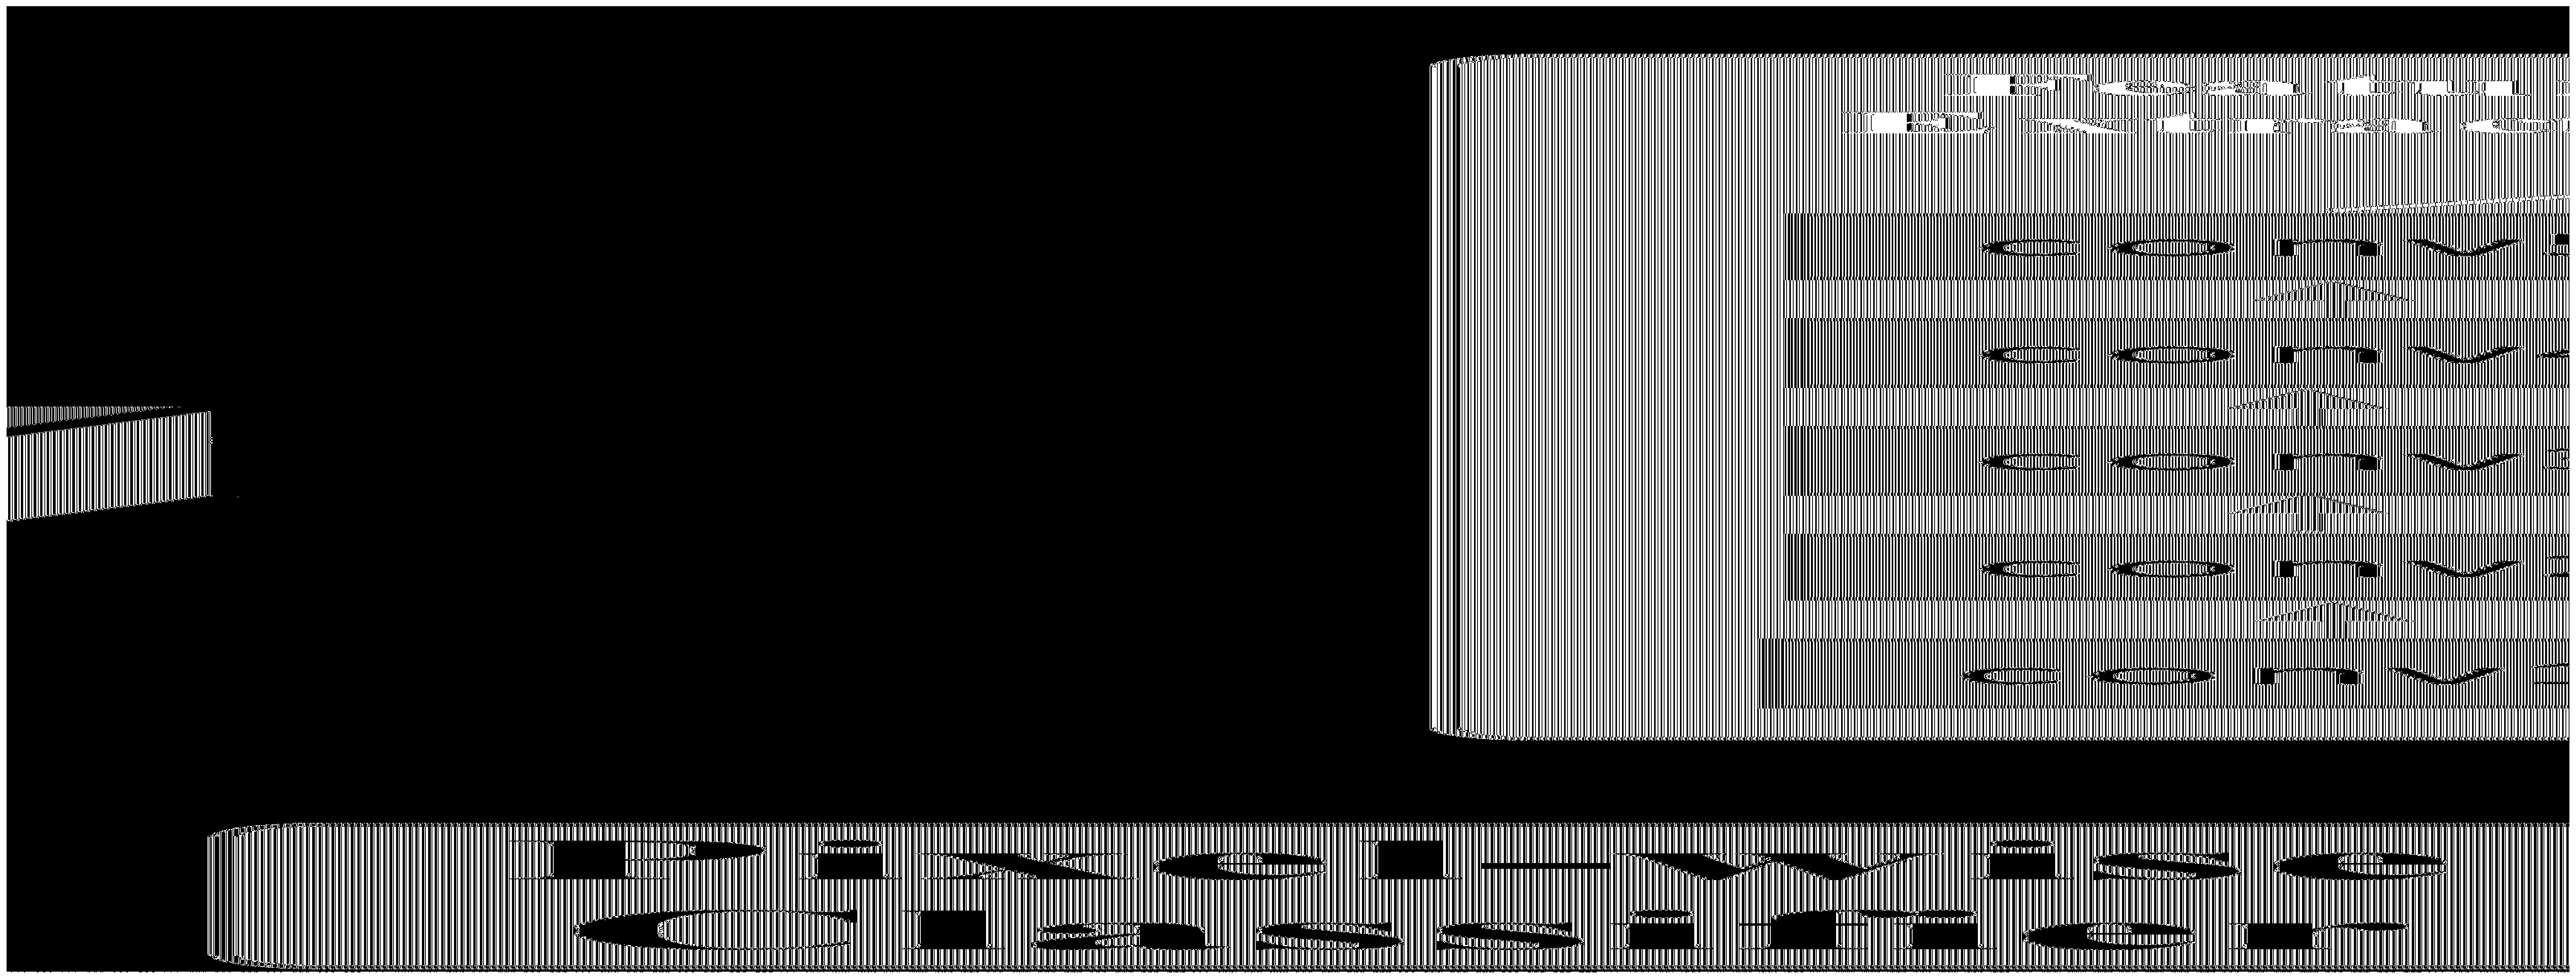
\includegraphics[width=134.79mm,height=50.80mm]{./CVPR2018_VideoSaliency_images/image004.eps.eps}

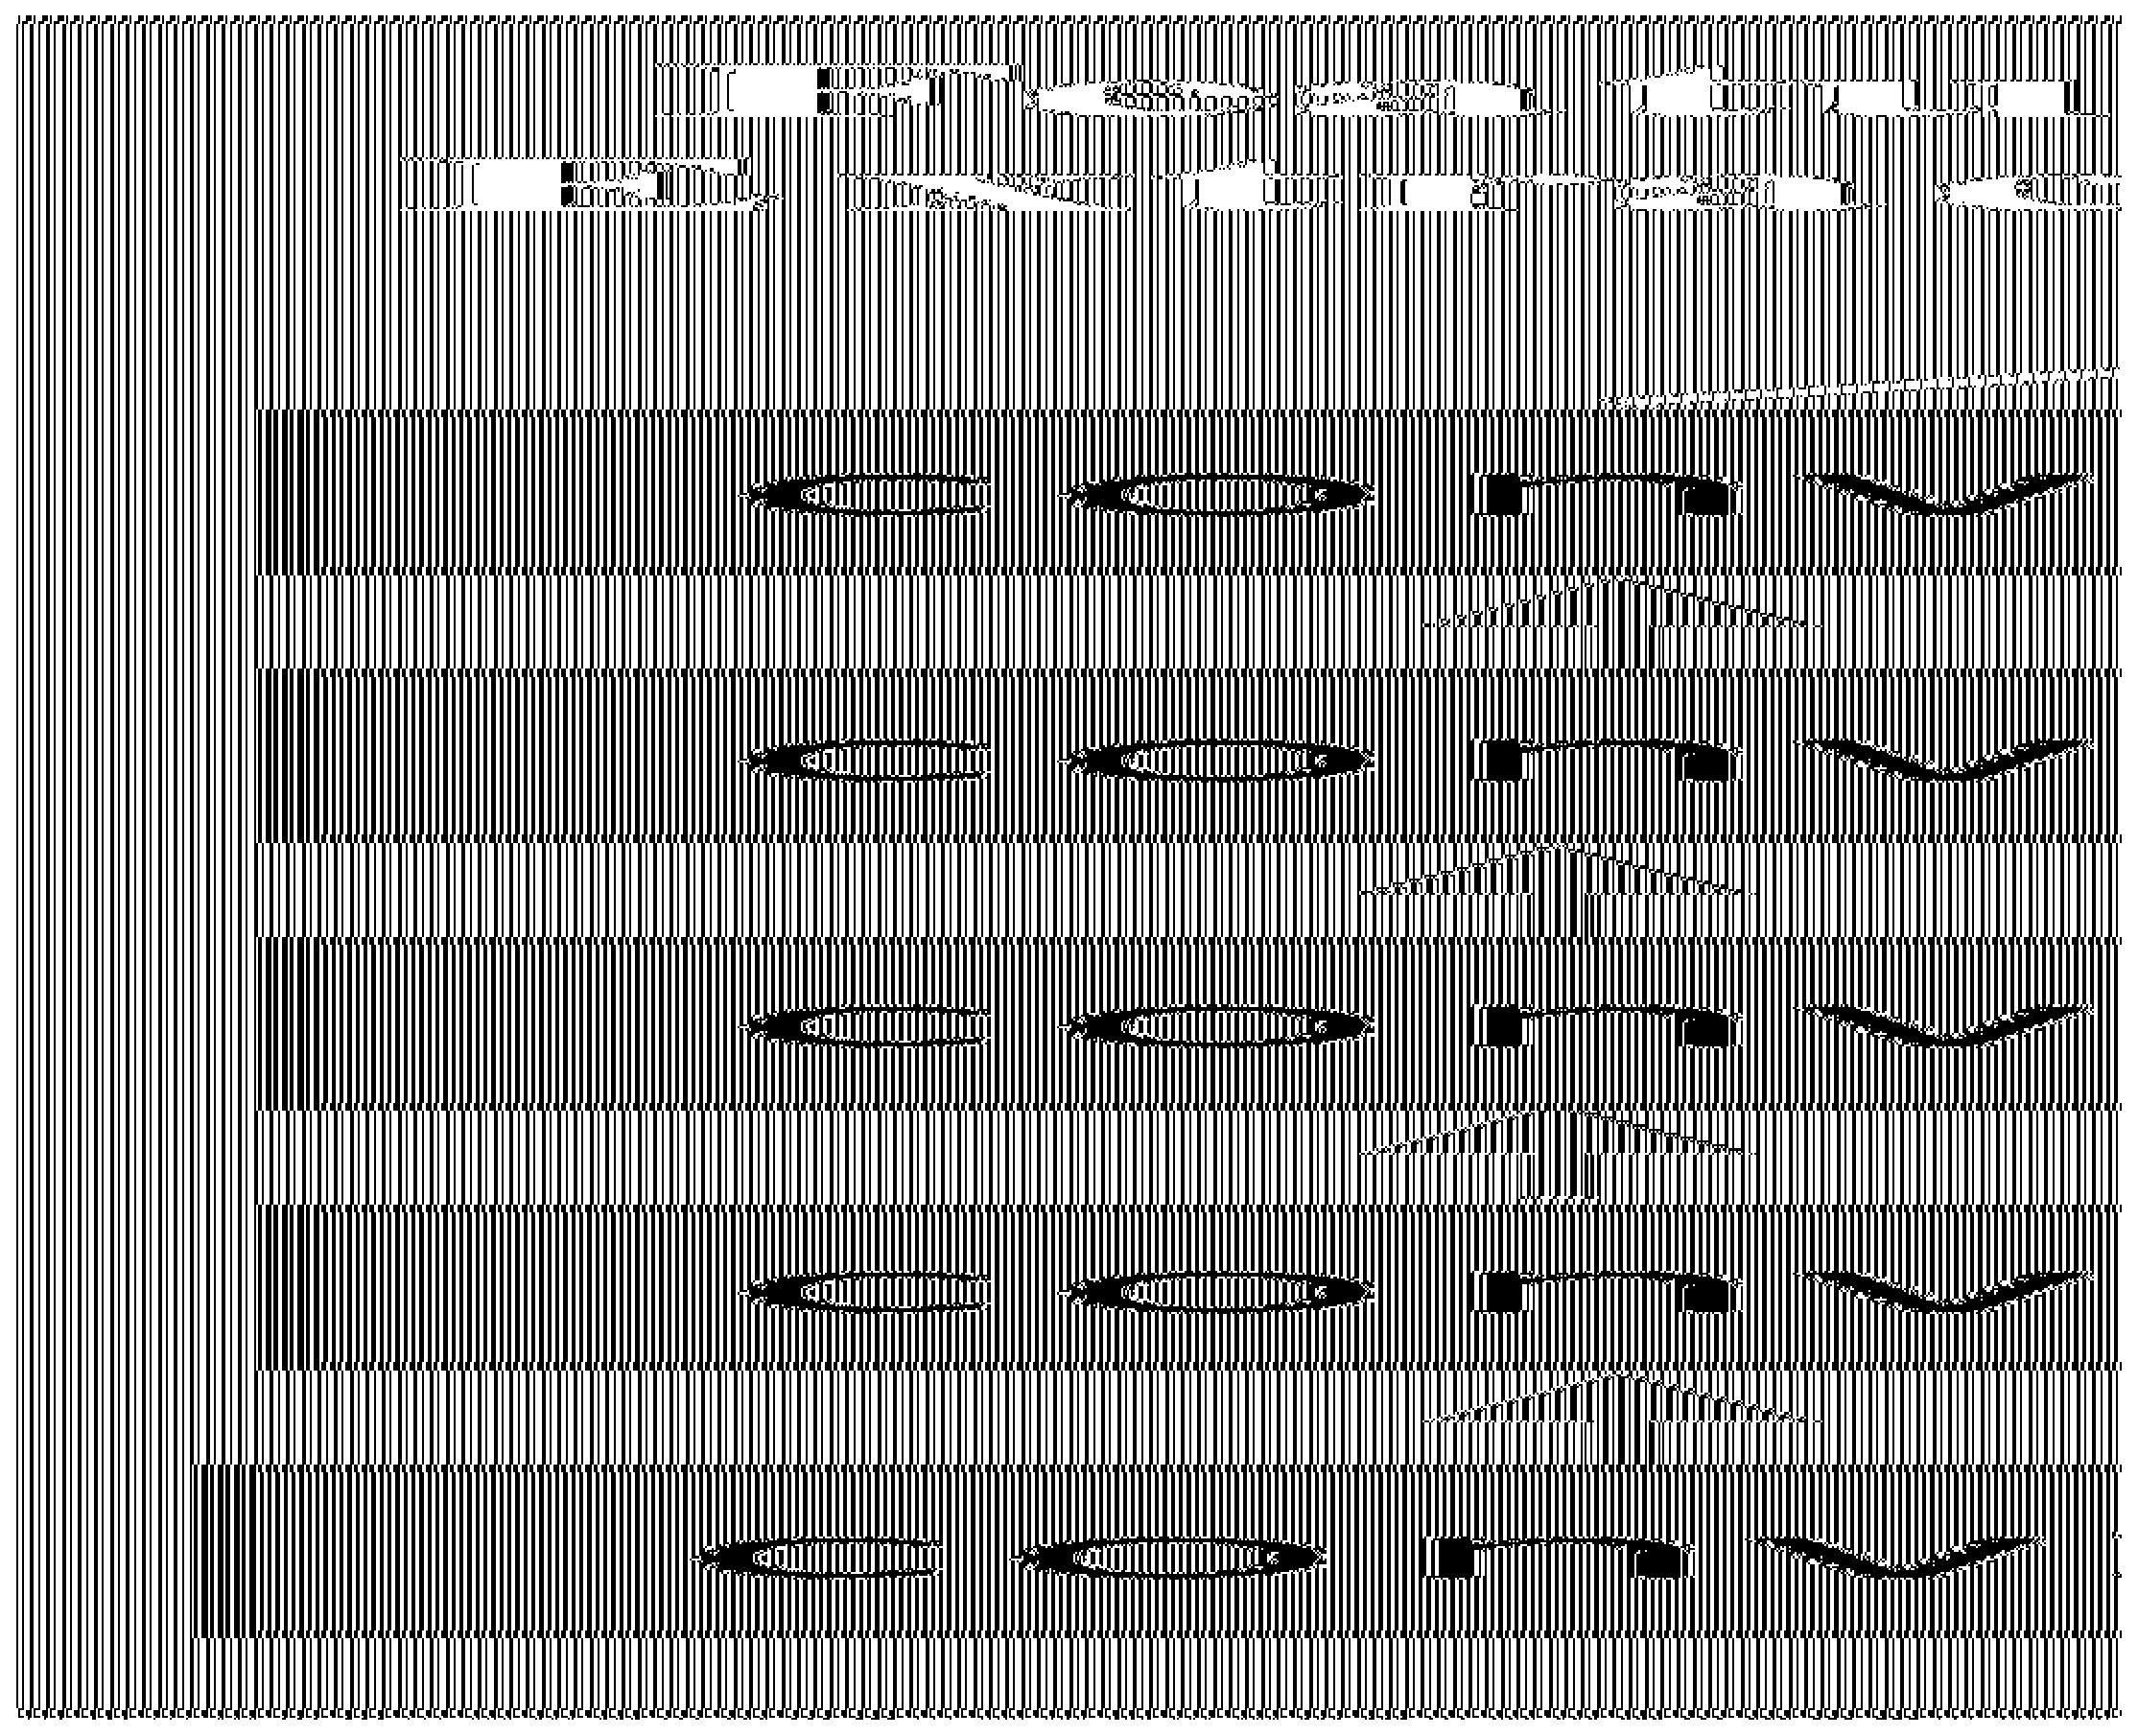
\includegraphics[width=44.62mm,height=36.11mm]{./CVPR2018_VideoSaliency_images/image005.eps.eps}
\end{center}
Figure2. Our overall framework for flow guided recurrent neural encoder. It incorporates a LSTM with reverse sequential input for motion flow update, a flow guided feature warping module and another LSTM for temporal coherence feature encoding.

coherence feature encoding, which produces the resulted feature $F_{i}$. The output saliency map is thus computed as $S_{i}=\mathcal{N}_{\mathrm{r}\mathrm{e}\mathrm{g}}(F_{i})$ .

3.1. Motion Computing and Updating

Given a reference $I_{i}$ and a window of $k$ former frames, we first apply the embedded FlowNet $\mathcal{F}[7]$ to individu- ally estimate $k$ initial flow fields $\{O_{i\rightarrow j}=\mathcal{F}(I_{i},\ I_{j})|j= i-1, i-2, i-k\}$ relative to the reference frame. The re- sulted flow field $O_{i\rightarrow j}$ is a position offset map of two chan- nels. It computes the pixel displacement $(u,\ v)$ for every pixel location $(x,\ y)$ in $I_{i}$ to the spatial location $(x',\ y')$ in $I_{j}$, i.e., $(x',\ y')=(x+u,\ y+v)$ , where $u$ and $v$ respec- tively represent the pixel offsets in horizontal and vertical directions.

As the FlowNet is originally trained from pair data of consecutive frames, it may not be accurate enough to reflect the motion relationship between two frames with long time interval. Intuitively, the closer to the reference frame, the more accurate the estimated motion flow. We can gradually employ flow maps of closer frames to refine that of larger time interval. Based on the above consideration, we propose to combine a ConvLSTM $[^{3}3^{9}9$] with CNN based FlowNet to jointly learn the flow map and refine in reverse order.

ConvLSTM is an extension of traditional fully con- nected LSTM which has convolutional structures in both input-to-state and state-to-state connections. All of the data transfered in ConvLSTM can be regarded as $3\mathrm{D}$ ten- sors with the last two dimensions being spatial dimen- sions. Let $\mathcal{X}_{1}, \mathcal{X}_{2}, \mathcal{X}_{t}$ denote the input to ConvLSTM and $\mathcal{H}_{1}, \mathcal{H}_{2}, \mathcal{H}_{t}$ stand for its hidden states. At each time step, the output hidden state of ConvLSTM is updated base on its own input as well as the encoded past states from its previous input, which is formulated as

$\mathcal{H}_{t}=$ConvLSTM , (1)

where $C$ is the memorized cell state of the ConvLSTM at its previous time-step. Following $[^{\fbox{$\mathrm{Error}::0\mathrm{x}0000$}}3^{(:}\fbox{$\mathrm{Error}::0\mathrm{x}0000$}.9$], the ConvLSTM mod- ule consists of the input gate $i_{t}$, forget gate $f_{t}$ and output gate $0_{t}$, the overall updating equations can be listed in (2), where $*$' denotes the convolution operator, `o' denotes the Hadamard product, and $\sigma$ stands for the sigmoid func- tion:

$i_{t}=\sigma(W_{xi}*\mathcal{X}_{t}+W_{hi}*\mathcal{H}_{t-1}+W_{ci}\circ C_{t-1}+b_{i})$

$f_{t}=\sigma(W_{xf}*\mathcal{X}_{t}+W_{hf}*\mathcal{H}_{t-1}+W_{cf}\circ C_{t-1}+b_{f})$

$C_{t}=f_{t}\circ C_{t-1}+i_{t}\circ\tanh(W_{xc}*\mathcal{X}_{t}+W_{hc}*\mathcal{H}_{t-1}+b_{c}) o_{t}=\sigma(W_{xo}*\mathcal{X}_{t}+W_{ho}*\mathcal{H}_{t-1}+W_{co}\circ C_{t-1}+b_{o})$

$\mathcal{H}_{t}=o_{t}\tanh(C_{t})$

(2)

To update the optical flow field with ConvLSTM, the LSTM layer is unrolled for awindow of $k$ flow fields and the size of the hidden state is set to be the same as the in- put flow map. We sequentially feed the $k$ initial motion flow to the ConvLSTM cells in reverse order, i.e., $\mathcal{X}_{1:k}= O_{i\rightarrow(i-1)}, O_{i\rightarrow(i-2)}, O_{i\rightarrow(i-k)}$. The hidden states are the encoding of the updated flow field, which is further fed to a convolutional layer with kernel size of $1\times 1$ to produce the refined flow map $RO_{i\rightarrow j}$, formulated as:
$$
j=i-t
$$
$\mathcal{H}_{t}=$ConvLSTM $O_{i\rightarrow j})$ (3)
$$
RO_{i\rightarrow j}=\mathrm{C}\mathrm{o}\mathrm{n}\mathrm{v}_{1\times 1}(\mathcal{H}_{t})
$$
3.2. Motion Guided Feature Warping

As motivated by $[4_{5}^{5\backslash }5)]$, given a refined flow map $RO_{i\rightarrow j},$ the feature maps $\mathcal{N}_{\mathrm{f}\mathrm{e}\mathrm{a}}(\mathrm{I})$ on the $j^{th}$ frame are warped to the reference frame by applying the following warping func- tion,
\begin{center}
$\mathrm{W}\mathrm{a}\mathrm{r}\mathrm{p}\mathrm{F}_{i\rightarrow j}=\mathcal{W}(\mathcal{N}_{\mathrm{f}\mathrm{e}\mathrm{a}}(I_{j}),\ RO_{i\rightarrow j})$   (4)
\end{center}
where $\mathrm{W}\mathrm{a}\mathrm{r}\mathrm{p}\mathrm{F}_{i\rightarrow j}$ refers to the feature maps warped from frame $j$ to frame $i. \mathcal{W}$ is the bilinear warping function,

evaluate our trained model on the testing sets of DAVIS and

FBMS.

which is applied on all the spatial locations for each channel of the feature maps. It is implemented as a bilinear interpo- lation of $\mathcal{N}_{\mathrm{f}\mathrm{e}\mathrm{a}}(\mathrm{I})$ at the desired positions w.r.t the optical flow $RO_{i\rightarrow j}.$

3.3. Temporal Coherence Feature Encoding

Although feature warping operation can compensate for the misalignment of features caused by object or camera motion. It is still not enough to characterize the continuous dynamic evolution of video frames as well as the evolution of appearance contrast in temporal domain. Base on the above considerations, we proposed to exploit another ConvLSTM for sequential feature encoding. Specifically, this ConvLSTM takes a sequence of warped features (including the feature of the reference frame) as input, i.e., $\mathcal{X}_{1:k}$ denoted in Equation (1) is set to $\mathcal{X}_{1:k}= \mathrm{W}\mathrm{a}\mathrm{r}\mathrm{p}\mathrm{F}_{i\rightarrow(i-k)}, \mathrm{W}\mathrm{a}\mathrm{r}\mathrm{p}\mathrm{F}_{i\rightarrow(i-k+1)}, \mathrm{W}\mathrm{a}\mathrm{r}\mathrm{p}\mathrm{F}_{i\rightarrow(i-1)},\mathcal{N}_{\mathrm{f}\mathrm{e}\mathrm{a}}(I_{i})$ , and works by computing the forward hidden sequence for temporal feature encoding from $t=1$ to $t=k+1$, and then updating the output layer. The state updating function in (1) can be rewritten as follows:

$j=i-k+(t-1)$

$\mathcal{H}_{t}=$ConvLSTM ($\mathcal{H}_{t-1},\ C_{t-1},\ \mathrm{W}\mathrm{a}\mathrm{r}\mathrm{p}\mathrm{F}_{i\rightarrow j}), t\leq k$ (5)

$\mathcal{H}_{k+1}=$ConvLSTM $(;_{;}\mathcal{N}_{\mathrm{f}\mathrm{e}\mathrm{a}}(I))$

The hidden states are the encoding of the memorized future till now. And the hidden state of the last time-step $k+1$ is our final feature encoding.

4. Experimental Results 4.1. Experimental Setup 4.1.1 Datasets

We evaluate the performance of our method on two public datasets: Freiburg-Berkeley Motion Segmentation (FBMS) dataset $[.2,\ 2_{5}^{5\backslash }5$)], and DAVIS $[2^{\cdot}7]$ dataset. The FBMS dataset contains 59 videos with 720 annotated sparsely annotated frames. DAVIS is a newly developed dataset for video ob- ject segmentation, which contains 50 high quality and full HD video sequences with 3,455 densely annotated pixel- level and per-frame ground-truth. It is one of the most chal- lenging benchmark which covers various video object seg- mentation challenges such as occlusions, motion blur and appearance changes.

There exists another dataset SegTrack V2, which is an extended dataset from the original SegTrack dataset pro- posed in $[..33\{_{\ovalbox{\tt\small REJECT}}.0$] and contains 14 videos about bird, animal, car and human with 1,066 densely annotated frame images. As referred to $[^{\fbox{$\mathrm{Error}::0\mathrm{x}0000$}}36_{\backslash }\cdot.6$], we combine the whole $\mathrm{S}\mathrm{e}\mathrm{g}\mathrm{T}\mathrm{r}\mathrm{a}\mathrm{c}\mathrm{k}\mathrm{V}2$, the training sets of FBMS and DAVIS as our training set, and

4.1.2 Evaluation Criteria

Similar to image-based salient object detection, we adopt precision-recall curves (PR), maximum $\mathrm{F}$-measure and mean absolute error (MAE) as the evaluation metrics. The continuous saliency map is rescaled to $[0,255]$ and is bina- rized using all integer thresholds in the interval. At each threshold value, a pair of precision and recall value can be obtained by comparing the binary saliency map against the groundtruth. The PR curve is obtained from the average precision and recall over saliency maps of all images in the dataset. The $\mathrm{F}$-measure is defined as
\begin{center}
$F_{\beta}=\displaystyle \frac{(1+\beta^{2})\cdot Precision\cdot Recall}{\beta^{2}\cdot Precision+Recall}$,   (6)
\end{center}
where $\beta^{2}$ is set to 0.3 as suggested in [1.]. We report the maximum $\mathrm{F}$-measure $($maxF) computed from the PR curve. MAE is defined as the average pixelwise absolute difference between the binary ground truth $G$ and the saliency map $S[26],$

4.1.3 Implementation Details

Our proposed FRGNE has been implemented on the Mxnet [{\it 4}], a flexible open source deep learning frame net- work. FGRNE is compatible with any FCN based still- image salient object detectors. In this paper, we choose the state-of-the-art deeply supervised salient object detec- tion (DSS) $[1.4_{\ovalbox{\tt\small REJECT}}.0]$ method with public trained model as a baseline and take the updated DSS with FGRNE embedded as our final model for video salient object detection when performing ablation study and compared with other bench- marks. In Section 4.3, we will list more results of our pro- posed FGRNE on other host networks to demonstrate the ef- fectiveness of our proposed algorithm. During training, the frame images are resized to 256$*$512 before feeding into the network. While inference, we resize the image to a shorter side of 256 pixels. We train all the components incorporated in our framework in an end-to-end mode using SGD with a momentum of 0.9. The learning rate is initially set to 2.5e- 4 and decayed by 0.9 at every $8\mathrm{k}$ training round. The loss function is set as same as the host network (e.g. DSS $[1.4_{-}0]$ employs an image-level class-balanced cross-entropy loss). The window size $k$ is limited by the memory, with its default value set to 5 in our experiment. We have also explored the impact of different settings in Section 4.3. Experiments are performed on a workstation with an NVIDIA Titan X GPU and a 3. $4\mathrm{G}\mathrm{H}\mathrm{z}$ Intel processor.
\begin{center}
\begin{tabular}{|l|l|l|l|l|l|l|l|l|l|l|l|}
\hline
\multicolumn{1}{|l|}{DATASET}&	\multicolumn{1}{|l|}{Metric}&	\multicolumn{1}{|l|}{MST}&	\multicolumn{1}{|l|}{$\mathrm{M}\mathrm{B}+$}&	\multicolumn{1}{|l|}{RFCN}&	\multicolumn{1}{|l|}{DHSNet}&	\multicolumn{1}{|l|}{DCL}&	\multicolumn{1}{|l|}{DSS}&	\multicolumn{1}{|l|}{SAG}&	\multicolumn{1}{|l|}{GF}&	\multicolumn{1}{|l|}{DLVSD}&	\multicolumn{1}{|l|}{FGRNE}	\\
\hline
&	\multicolumn{1}{|l|}{$\mathrm{m}\mathrm{a}\mathrm{x}\mathrm{F}$}&	\multicolumn{1}{|l|}{ $0.455$}&	\multicolumn{1}{|l|}{ $0.520$}&	\multicolumn{1}{|l|}{ $0.732$}&	\multicolumn{1}{|l|}{ $0.778$}&	\multicolumn{1}{|l|}{ $0.740$}&	\multicolumn{1}{|l|}{ $0.775_{\fbox{$\mathrm{Error}::0\mathrm{x}0000$}}^{\ovalbox{\tt\small REJECT}}5$}&	\multicolumn{1}{|l|}{ $0.528$}&	\multicolumn{1}{|l|}{ $0.628$}&	\multicolumn{1}{|l|}{ $0.699$}&	\multicolumn{1}{|l|}{ $0.798$}	\\
\cline{2-12}
&	\multicolumn{1}{|l|}{MAE}&	\multicolumn{1}{|l|}{$0.165$}&	\multicolumn{1}{|l|}{ $0.183$}&	\multicolumn{1}{|l|}{ $0.047$}&	\multicolumn{1}{|l|}{ $0.035$}&	\multicolumn{1}{|l|}{ $0.061$}&	\multicolumn{1}{|l|}{ $0.047$}&	\multicolumn{1}{|l|}{ $0.080$}&	\multicolumn{1}{|l|}{ $0.067$}&	\multicolumn{1}{|l|}{ $0.064$}&	\multicolumn{1}{|l|}{ $0.032$}	\\
\cline{2-12}
\multicolumn{1}{|l|}{ $\mathrm{F}\mathrm{T}\mathrm{i}1l/|\mathrm{q}$}&	\multicolumn{1}{|l|}{ $\mathrm{m}\mathrm{a}\mathrm{x}\mathrm{F}$}&	\multicolumn{1}{|l|}{ $0.540$}&	\multicolumn{1}{|l|}{ $0.525$}&	\multicolumn{1}{|l|}{ $0.741$}&	\multicolumn{1}{|l|}{ $0.744$}&	\multicolumn{1}{|l|}{ $0.740$}&	\multicolumn{1}{|l|}{ $0.76_{6}^{6}0\ovalbox{\tt\small REJECT}$}&	\multicolumn{1}{|l|}{ $0.572$}&	\multicolumn{1}{|l|}{ $0.607$}&	\multicolumn{1}{|l|}{ $0.696$}&	\multicolumn{1}{|l|}{ $0.783$}	\\
\cline{2-12}
\multicolumn{1}{|l|}{ $\mathrm{I}\rightarrow\perp \mathrm{V}\mathrm{I}\cup$}&	\multicolumn{1}{|l|}{MAE}&	\multicolumn{1}{|l|}{$0.179$}&	\multicolumn{1}{|l|}{ $0.204$}&	\multicolumn{1}{|l|}{ $0.089$}&	\multicolumn{1}{|l|}{ $0.076$}&	\multicolumn{1}{|l|}{ $0.133$}&	\multicolumn{1}{|l|}{ $0.077$}&	\multicolumn{1}{|l|}{ $0.145$}&	\multicolumn{1}{|l|}{ $0.101$}&	\multicolumn{1}{|l|}{ $0.077$}&	\multicolumn{1}{|l|}{ $0.063$}	\\
\hline
\end{tabular}

\end{center}
Table 1. Comparison of quantitative results including maximum $\mathrm{F}$-measure (larger is better) and MAE (smaller is better). The best three results are shown in red, blue, and green, respectively.
\begin{center}
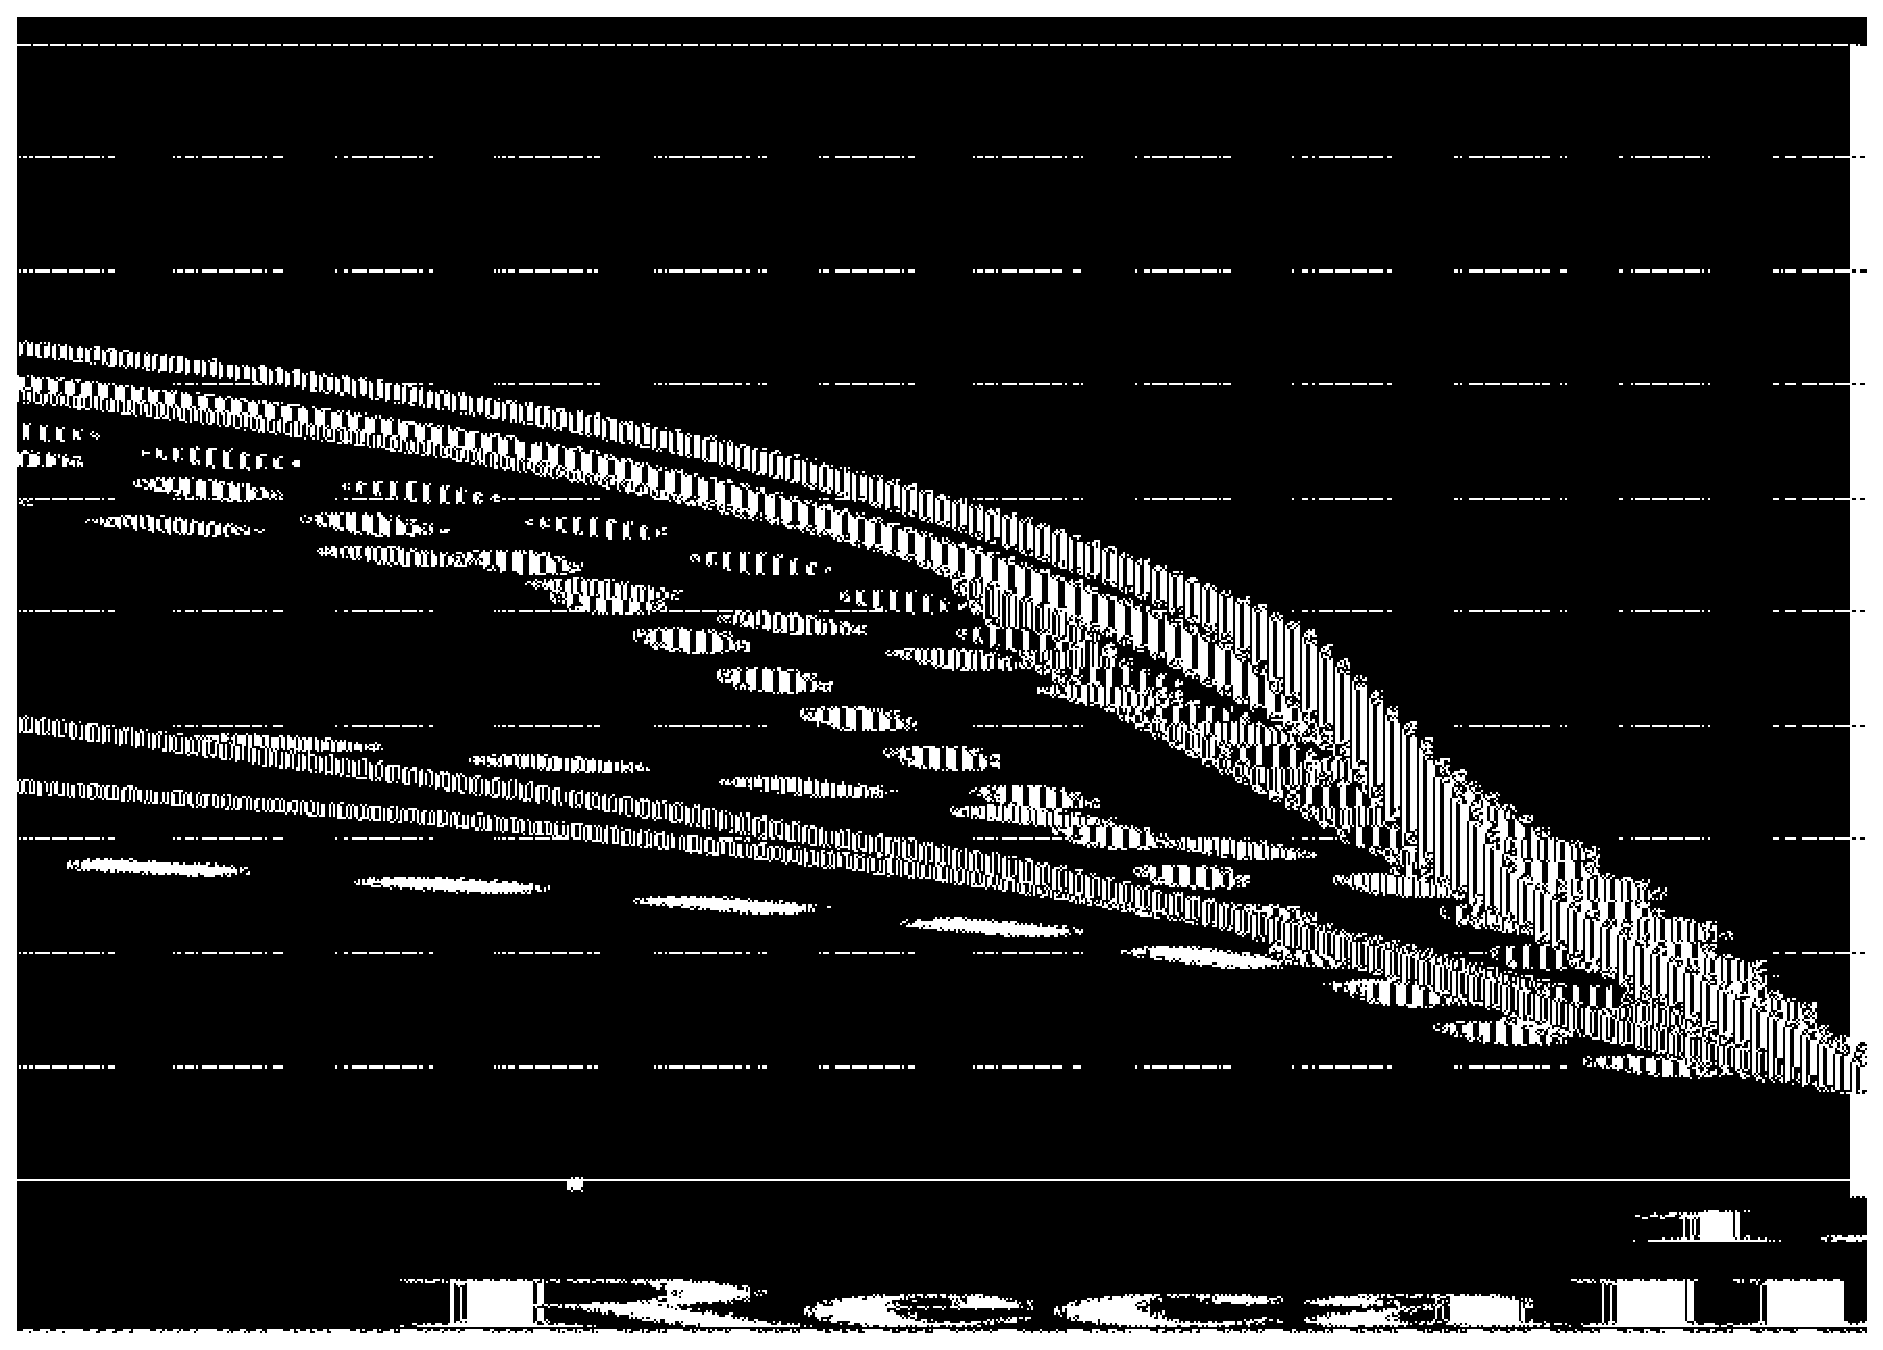
\includegraphics[width=37.59mm,height=26.75mm]{./CVPR2018_VideoSaliency_images/image006.eps.eps}

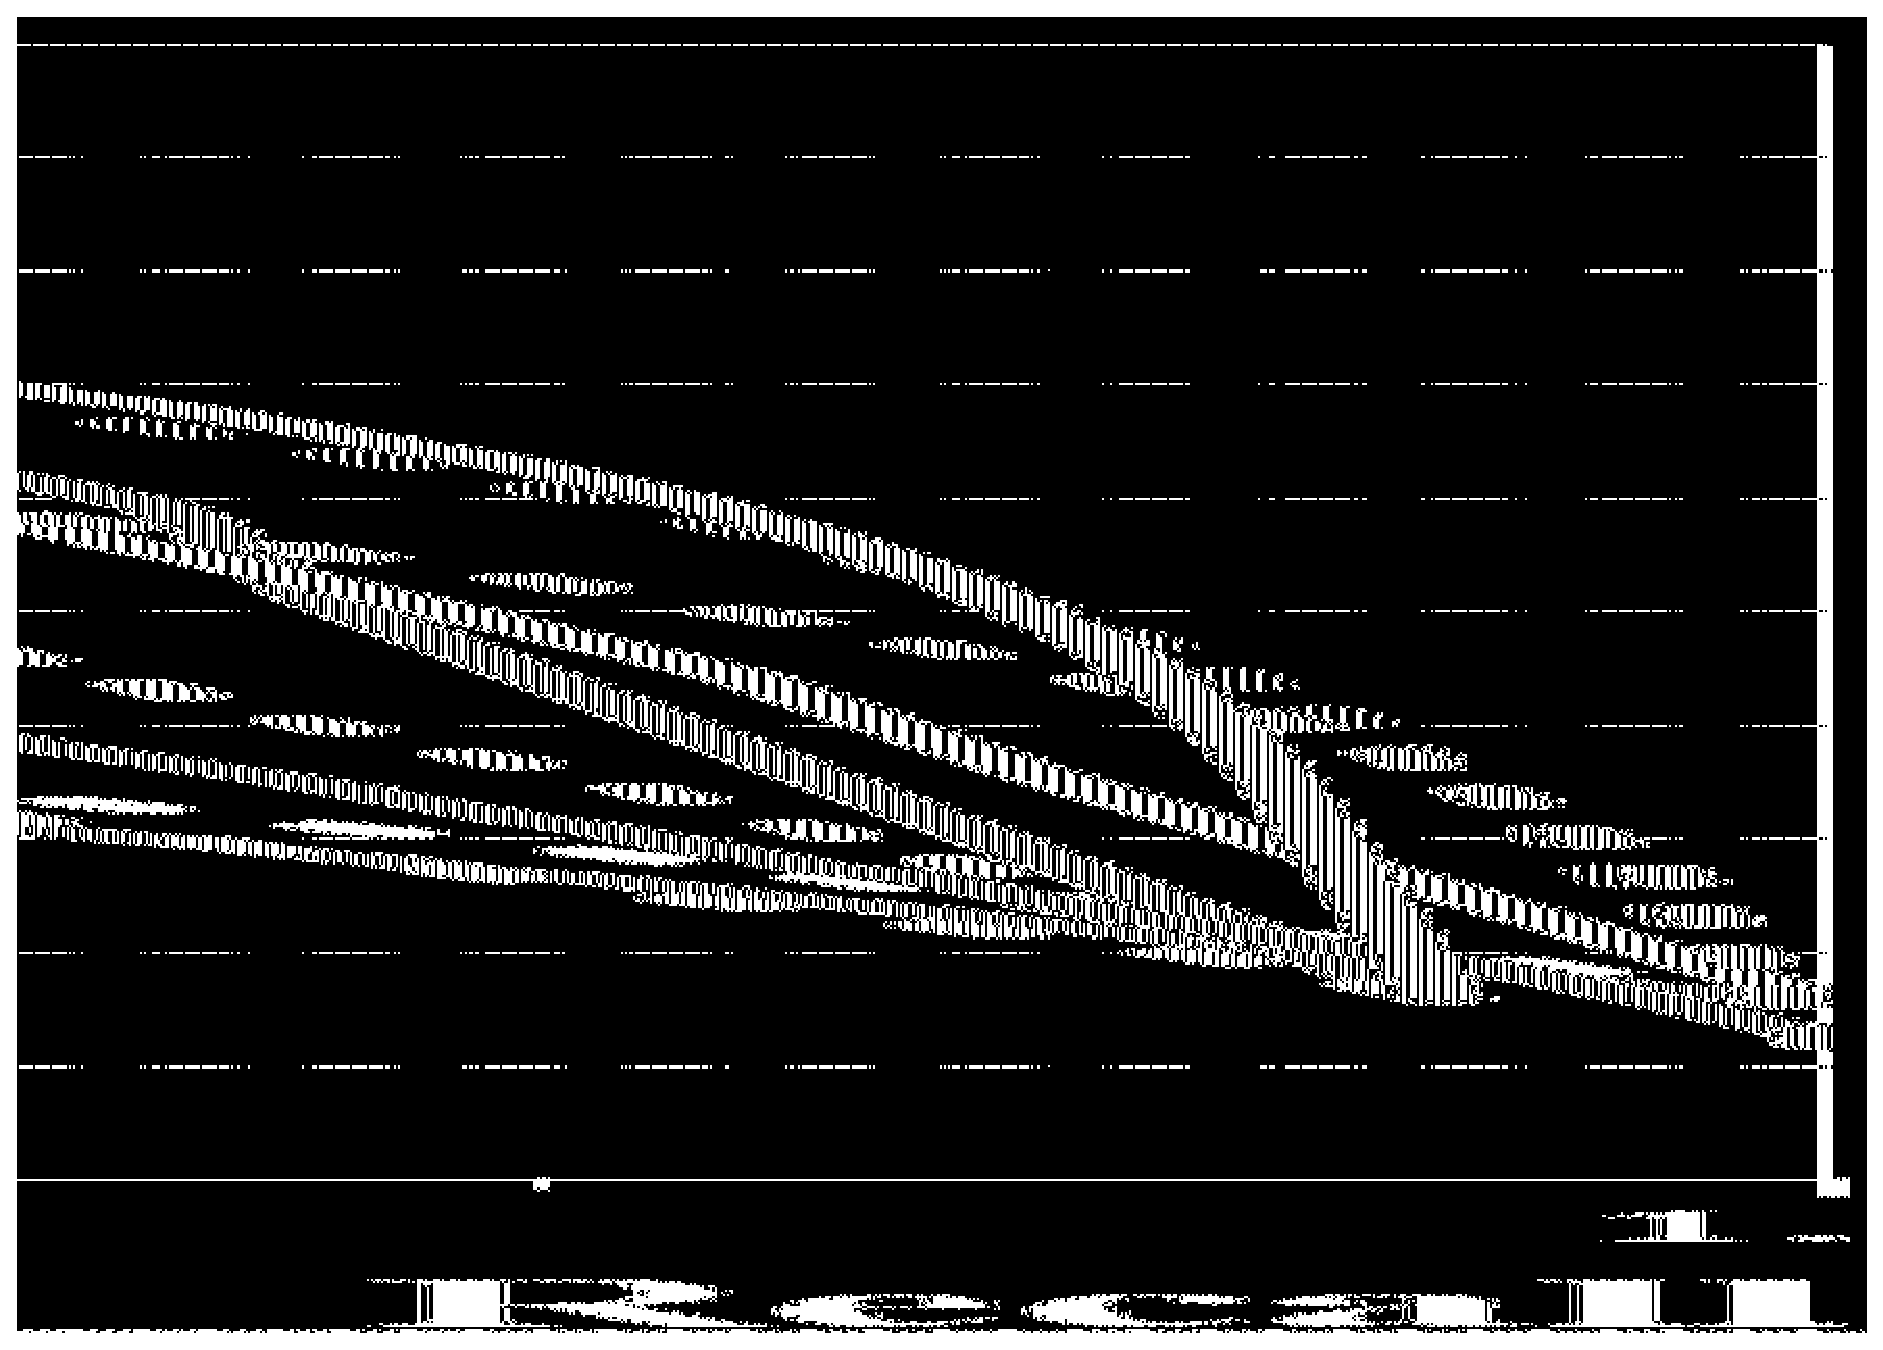
\includegraphics[width=37.59mm,height=26.75mm]{./CVPR2018_VideoSaliency_images/image007.eps.eps}
\end{center}
Figure 3. Comparison of precision-recall curves of 10 saliency de- tection methods on DAVIS and FBMS. Our proposed FGRNE con- sistently outperform other methods across the two testing dataset.

4.2. Comparison with the State of the Art

We compare our method (FGRNE) against 9 recent state-of-the-art methods, including MST $[^{3}31 \mathrm{M}\mathrm{B}+[\cdot 4_{\backslash }'41.],$

RFCN [..3..3], DHSNet $[2^{3}3]$, DCL [20], DSS [10], SAG $[^{3}34$], GF $[..3_{\fbox{$\mathrm{Error}::0\mathrm{x}0000$}}^{5}55]$ and DLVSD $[^{\fbox{$\mathrm{Error}::0\mathrm{x}0000$}}36_{\backslash }6$]. The first six are the latest state- of-the-art salient object detection methods for static images while the last three are video-based saliency models. For fair comparison, we use either the implementations or the saliency maps provided by the authors. We also fine-tune all the public static saliency models using the training set as same as we train our FGRNE, and use the refined model for comparison.

A visual comparison is illustrated in Fig. 4. As can be seen, deep learning based static saliency models can generate seemly promising saliency maps when watched independently, they are unsurprisingly inconsistent when putting in a whole sequence. Though existing video-based models can produce consistent results on videos with rela- tively slight object motions, they still can not handle videos with dramatic changes in appearance (object or camera mo- tion). It is particularly noteworthy that our proposed method incorporates the off-the-shelf DSS [1.0] model as our base- line, it can learn to improve the original feature with tempo- ral coherence and eventually produce optimized results far better than the original ones. In general, our method gen- erates much more accurate and consistent saliency maps in various challenging cases.

As a part of quantitative evaluation, we show a compar- ison of PR curves in Fig. 3. As shown in the figures, our method (FGRNE) significantly outperforms all state-of-the- art static and dynamic salient object detection algorithms on both DAVIS and FBMS. Moreover, a quantitative compari- son of maximum $\mathrm{F}$-measure and MAE is listed in Table. 1,

our proposed method improves the maximum $\mathrm{F}$-measure achieved by the best-performing static algorithm by 5.24\% and 2.57\% respectively on FBMS and DAVIS, and low- ers the MAE by 17.10\% and 8.57\% accordingly. When compared with the best-performing video-based model, our FGRNE improves the maximum $\mathrm{F}$-measure by 12.50\% and 14.16\% respectively on the FBMS and DAVIS dataset, and lowers the MAE by 18.18\% and 50\% accordingly. An in- teresting phenomenon is that the current best static saliency model actually outperforms the state-to-state video-based salient object detection methods because of the outstanding fully convolutional network.

Methods

feature aggregation?

flow guided feature warping?

flow update with LSTM?
\begin{center}
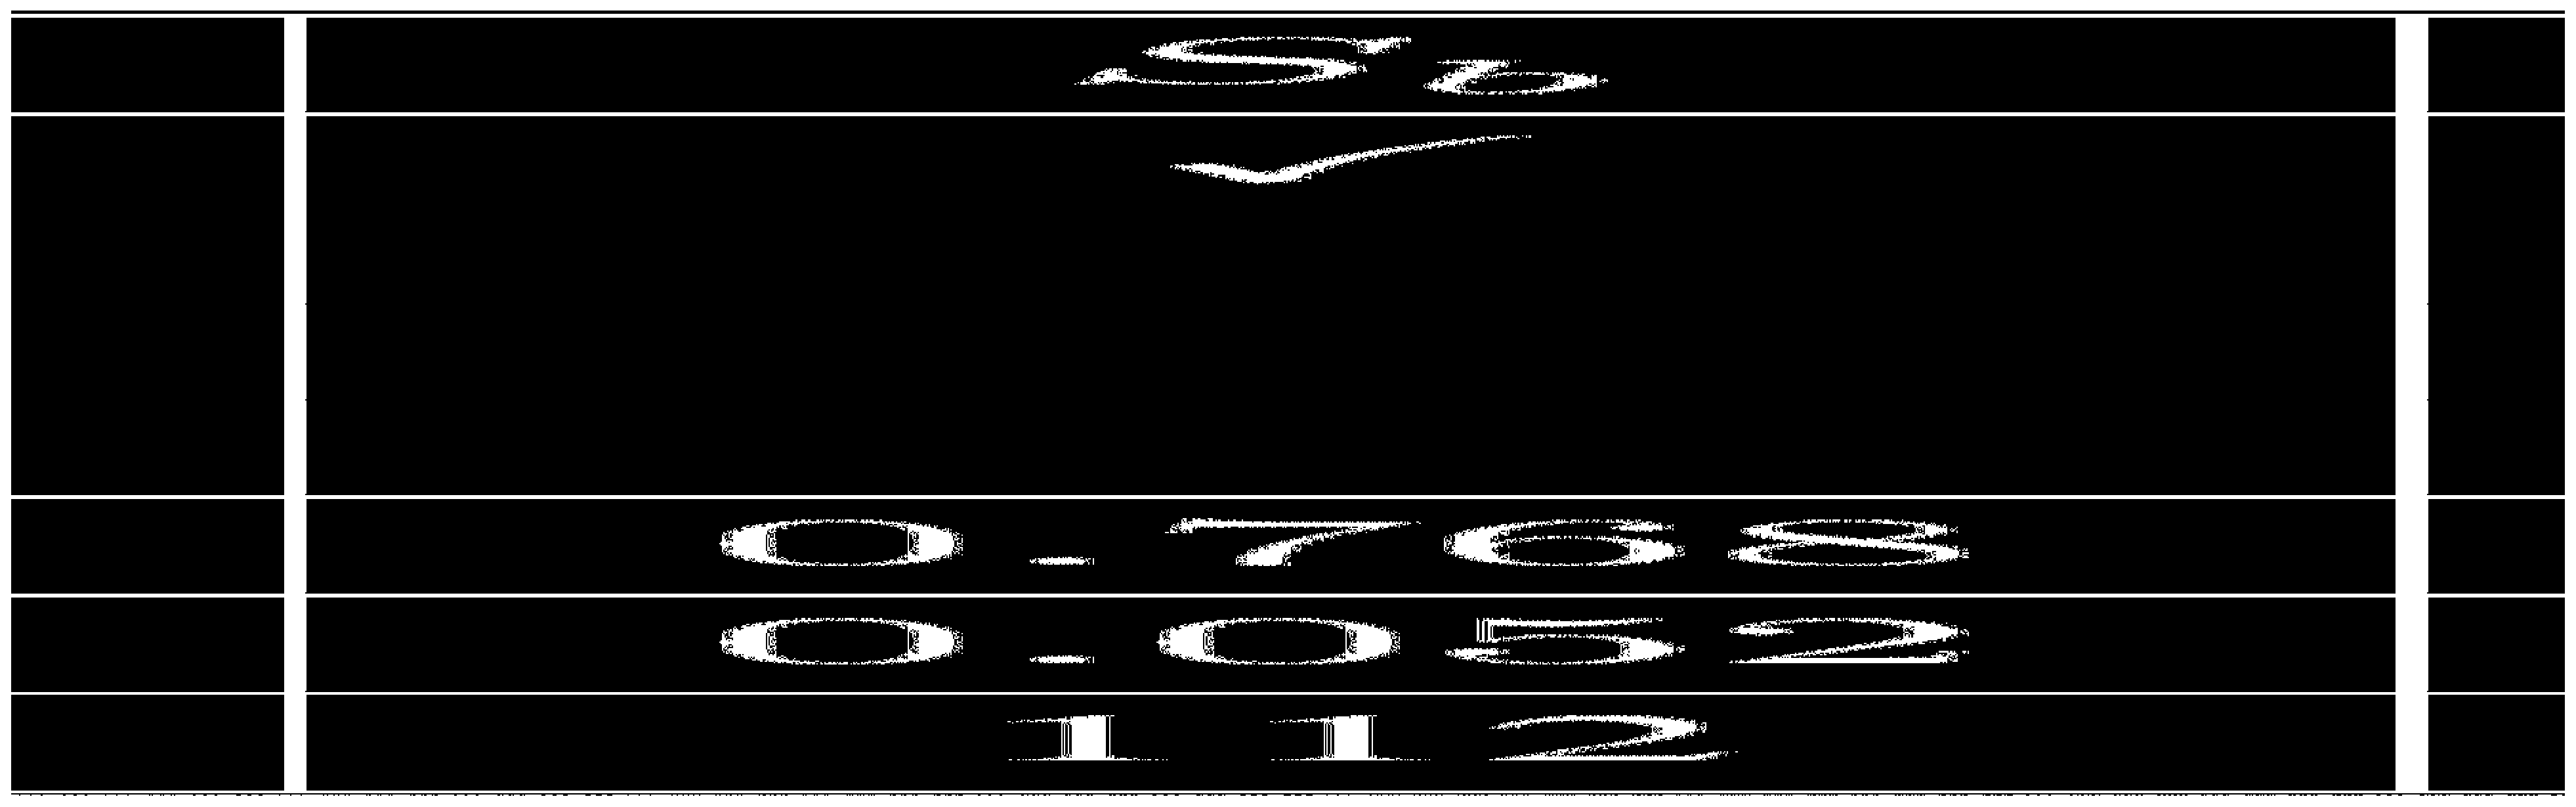
\includegraphics[width=79.08mm,height=24.30mm]{./CVPR2018_VideoSaliency_images/image008.eps.eps}
\end{center}
feature encoding with LSTM?

maxF MAE

0.775 0.047

0:798 0:032

runtime(ms)

97

0:768 0:052 112

0:777 0:036 137

0:780 0:036 162

0:793 0:035 184

191

Table 2. Effectiveness of flow guided recurrent neural encoder.

4.3. Ablation Studies

4.3.1 Effectiveness of Flow Guided Recurrent Neural Encoder

As discussed in Section 3, our proposed FGRNE involves three major modules, including motion flow updating, mo- tion guided feature warping and temporal coherence fea- ture encoding. To validate the effectiveness and necessity of each of these three modules, we compare FGRNE with its five variants in Table. 2.

$S_{a}$ refers to the saliency maps generated from the single- frame baseline model. To facilitate comparison, we also finetune the model using the individual frames of our used training set. It reaches the $\displaystyle \max F_{\beta}=$ 0:775 and MAE $=$ 0:047 in the test set of DAVIS, which already outperforms most of the state-of-the-art methods. This indicates that the fine-tuned baseline model is competitive and serves as a valid reference for evaluation. Compared to our en- tire framework, it is shown that embedding FGRNE to the baseline model totally leads to a 2.97\% $\mathrm{F}$-measure increase while reducing the MAE by 31.91\%.

$S_{b}$ refers to a naive feature aggregation algorithm on the baseline model. The feature of the reference frame is sim- ply updated as the weighted sum of the feature maps in
\begin{center}
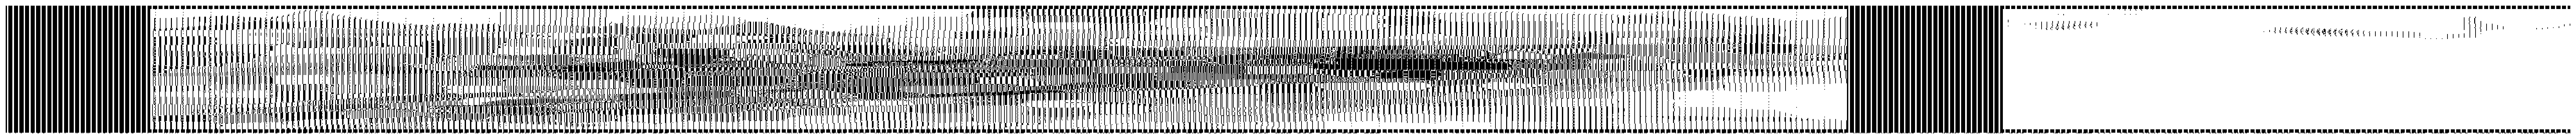
\includegraphics[width=156.13mm,height=7.79mm]{./CVPR2018_VideoSaliency_images/image009.eps.eps}

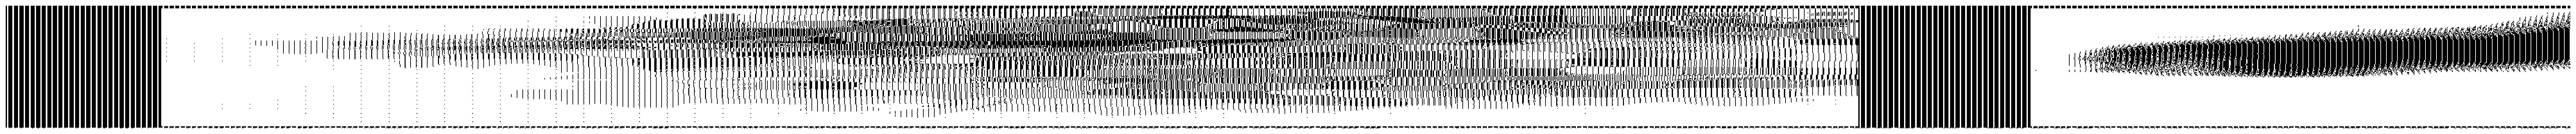
\includegraphics[width=156.13mm,height=7.45mm]{./CVPR2018_VideoSaliency_images/image010.eps.eps}

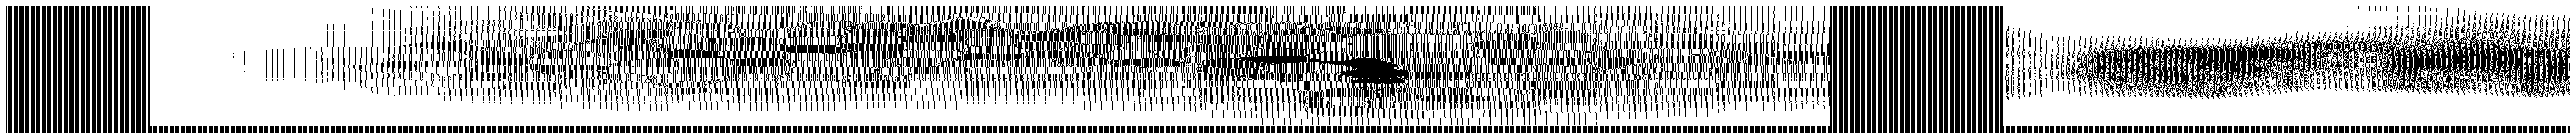
\includegraphics[width=156.13mm,height=7.79mm]{./CVPR2018_VideoSaliency_images/image011.eps.eps}

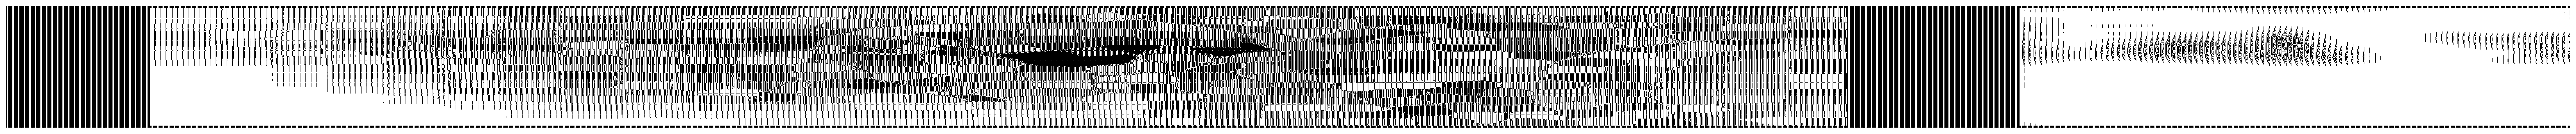
\includegraphics[width=156.13mm,height=7.45mm]{./CVPR2018_VideoSaliency_images/image012.eps.eps}

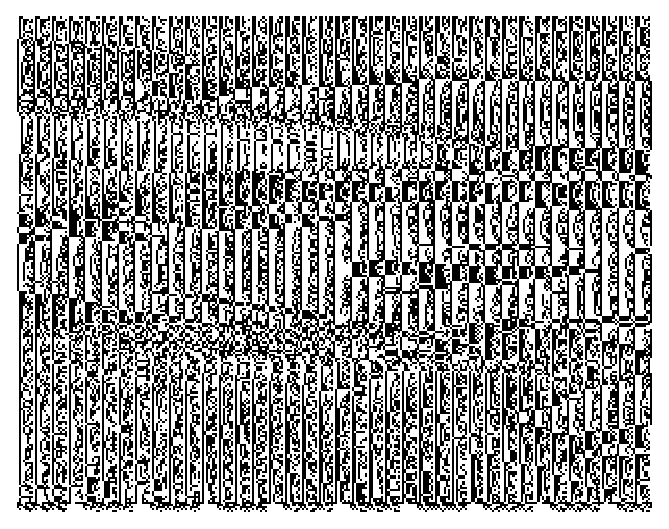
\includegraphics[width=12.91mm,height=10.08mm]{./CVPR2018_VideoSaliency_images/image013.eps.eps}

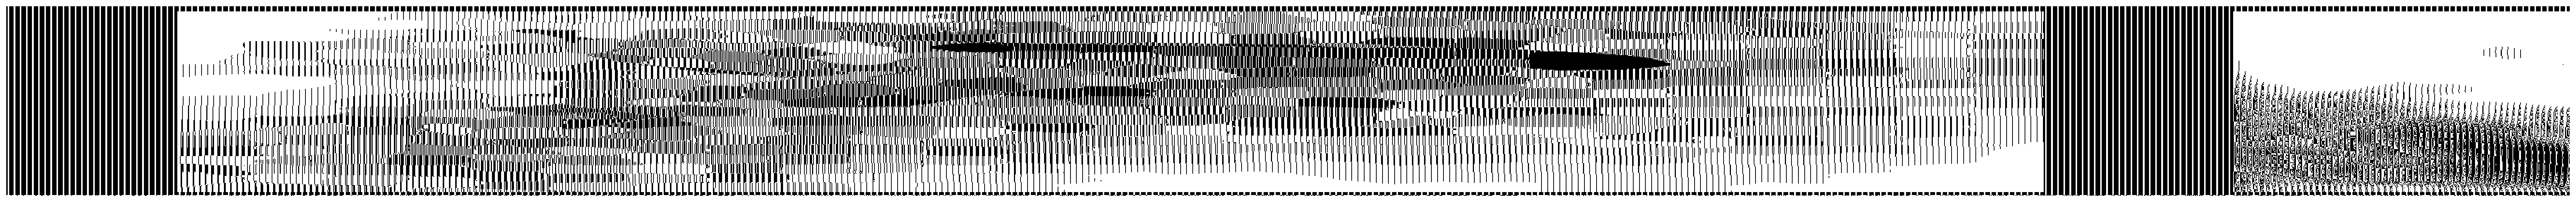
\includegraphics[width=141.90mm,height=10.50mm]{./CVPR2018_VideoSaliency_images/image014.eps.eps}

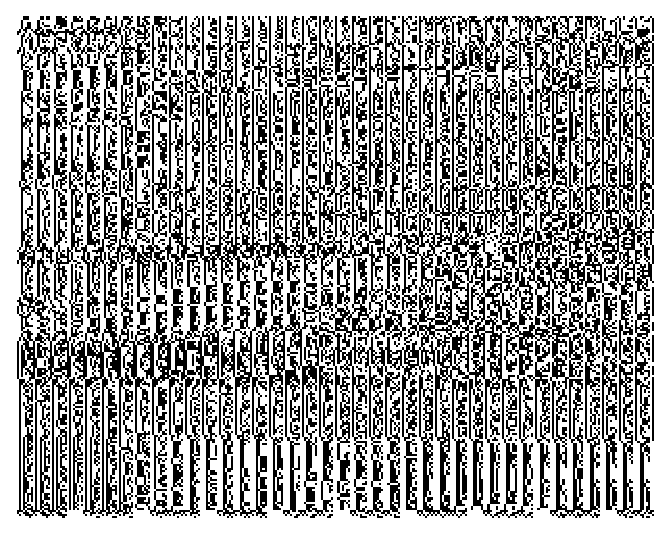
\includegraphics[width=12.95mm,height=10.20mm]{./CVPR2018_VideoSaliency_images/image015.eps.eps}

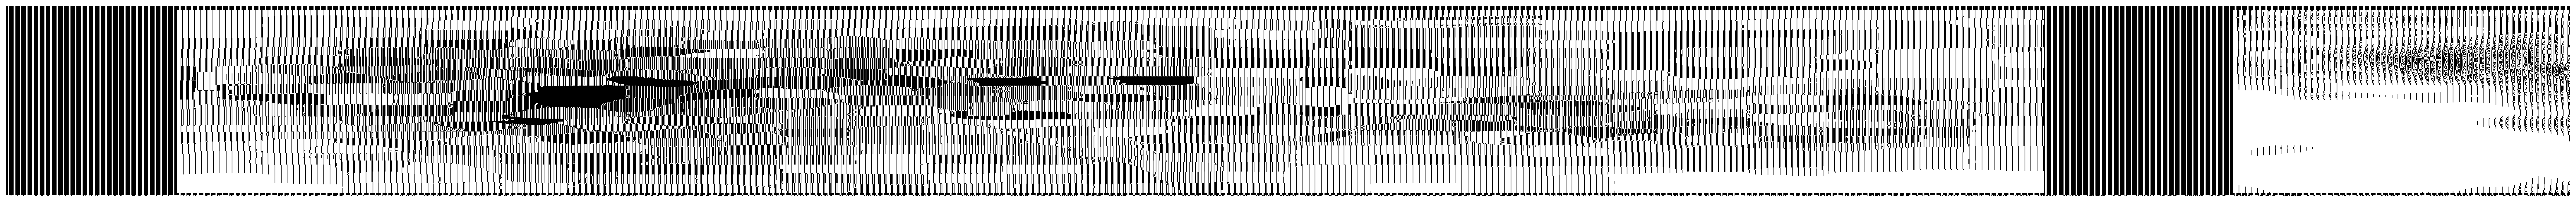
\includegraphics[width=141.90mm,height=10.50mm]{./CVPR2018_VideoSaliency_images/image016.eps.eps}
\end{center}
Figure 4. Visual comparison of saliency maps generated from state-of-the-art methods, including our FGRNE. The ground truth (GT) is shown in the last column. Our model consistently produces saliency maps closest to the ground truth.

the watching window, with the weight of $j^{th}$ frame $w_{i\rightarrow j}$ set to $\displaystyle \frac{1}{i-j+1}$. It is denoted as $F_{i}=\displaystyle \sum_{l=0}^{k}\frac{1}{l+1}\mathcal{N}_{\mathrm{f}\mathrm{e}\mathrm{a}}(F_{i-l})$ . It is also trained end-to-end in the same way as we train our FGRNE. As shown in the table, the $\mathrm{F}$-measure of this variant drops to 0:768 while the MAE increases to 0:052, which is even shy of the baseline model. It suggests that this naive feature aggregation is not suitable for sequential feature modeling. We speculate that the reason lies in the misalignment of features caused by changes in scene struc- ture and appearance.

$S_{c}$ refers to a simple feature encoding algorithm on the baseline model, and a degenerate variant of FGRNE. The motion updating module is turned off and no flow motion is used, i.e., the motion flow $O_{i\rightarrow j}$ is set to all zeros dur- ing training. The variant is also trained end-to-end in the same way as FGRNE. As shown in the table, the $\mathrm{F}$-measure obtains a very slight increase to 0:777, while MAE greatly decreases by 23.40\% to 0:036. However, the performance is still much inferior to the proposed FGRNE. This indicates that recurrent neural encoder can learn to exploit feature of previous frames to improve the temporal coherence of the reference frame. However, LSTM based feature encoding alone is not enough.

$S_{d}$ adds motion guided feature warping to the model of $S_{b}$, without the motion evolution update module turned on. It is actually a flow guided feature aggregation program. It increases the $\mathrm{F}$-measure by 1.56\% to 0.780 while lowers the MAE by 30.77\% to 0.036 w.r.t the performance of $S_{b}.$ It implies that feature alignment is an important operation before feature aggregation. The evident performance gain towards that of $S_{a}$ also reveals the importance of motion modeling for video salient object detection.

$S_{e}$ adds motion guided feature warping to the model of

$S_{c}$. It is a degenerate version of FGRNE without motion flow updating. All the other factors remain the same. It in- creases the $\displaystyle \max \mathrm{F}$-measure by 2.06\% to 0:793 and lowers the MAE by 2.78\% to 0.035 w.r.t the performance of $S_{c},$ which implies that the performance gain of motion guided feature warping is complementary to the LSTM based tem- poral coherence modeling. In fact, both object motion and the change of its appearance contrast are two core influenc- ing factors to video saliency, which correspond exactly to the design of two complementary modules in our proposed

FGRNE.

$S_{f}$ refers to the proposed FGRNE method, which turns on the motion flow evolution update module in $S_{e}$. It fur- ther brings a 0.63\% boost to the $\mathrm{F}$-measure to 0:798 while reducing the MAE by 8.57\% to 0:032. This demonstrate the reverse LSTM can help to refine the motion flow, which makes up for the lack of FlowNet in estimating optical flow for frame pairs with large time interval.

Moreover, we have also listed the comparison on runtime cost of each variant of our proposed FGRNE. As shown in the figure, incorporating FGRNE to a static model cost an extra $94\mathrm{m}\mathrm{s}$ per-frame. Noted that the feature extraction are shared during the saliency inference of all the frames in a given window and our algorithm runs in a sliding window mode. Therefore, enlarging the window size does not con- tribute to severe increase of time computation cost.

4.3.2 Sensitivities to Feature Extractor Selection

As described in Section 3, our FGRNE is dependent on a pre-trained static saliency detector as our host network. The host network is split into a feature extractor and a pixel-wise classification module. In principle, it can be split at any
\begin{center}
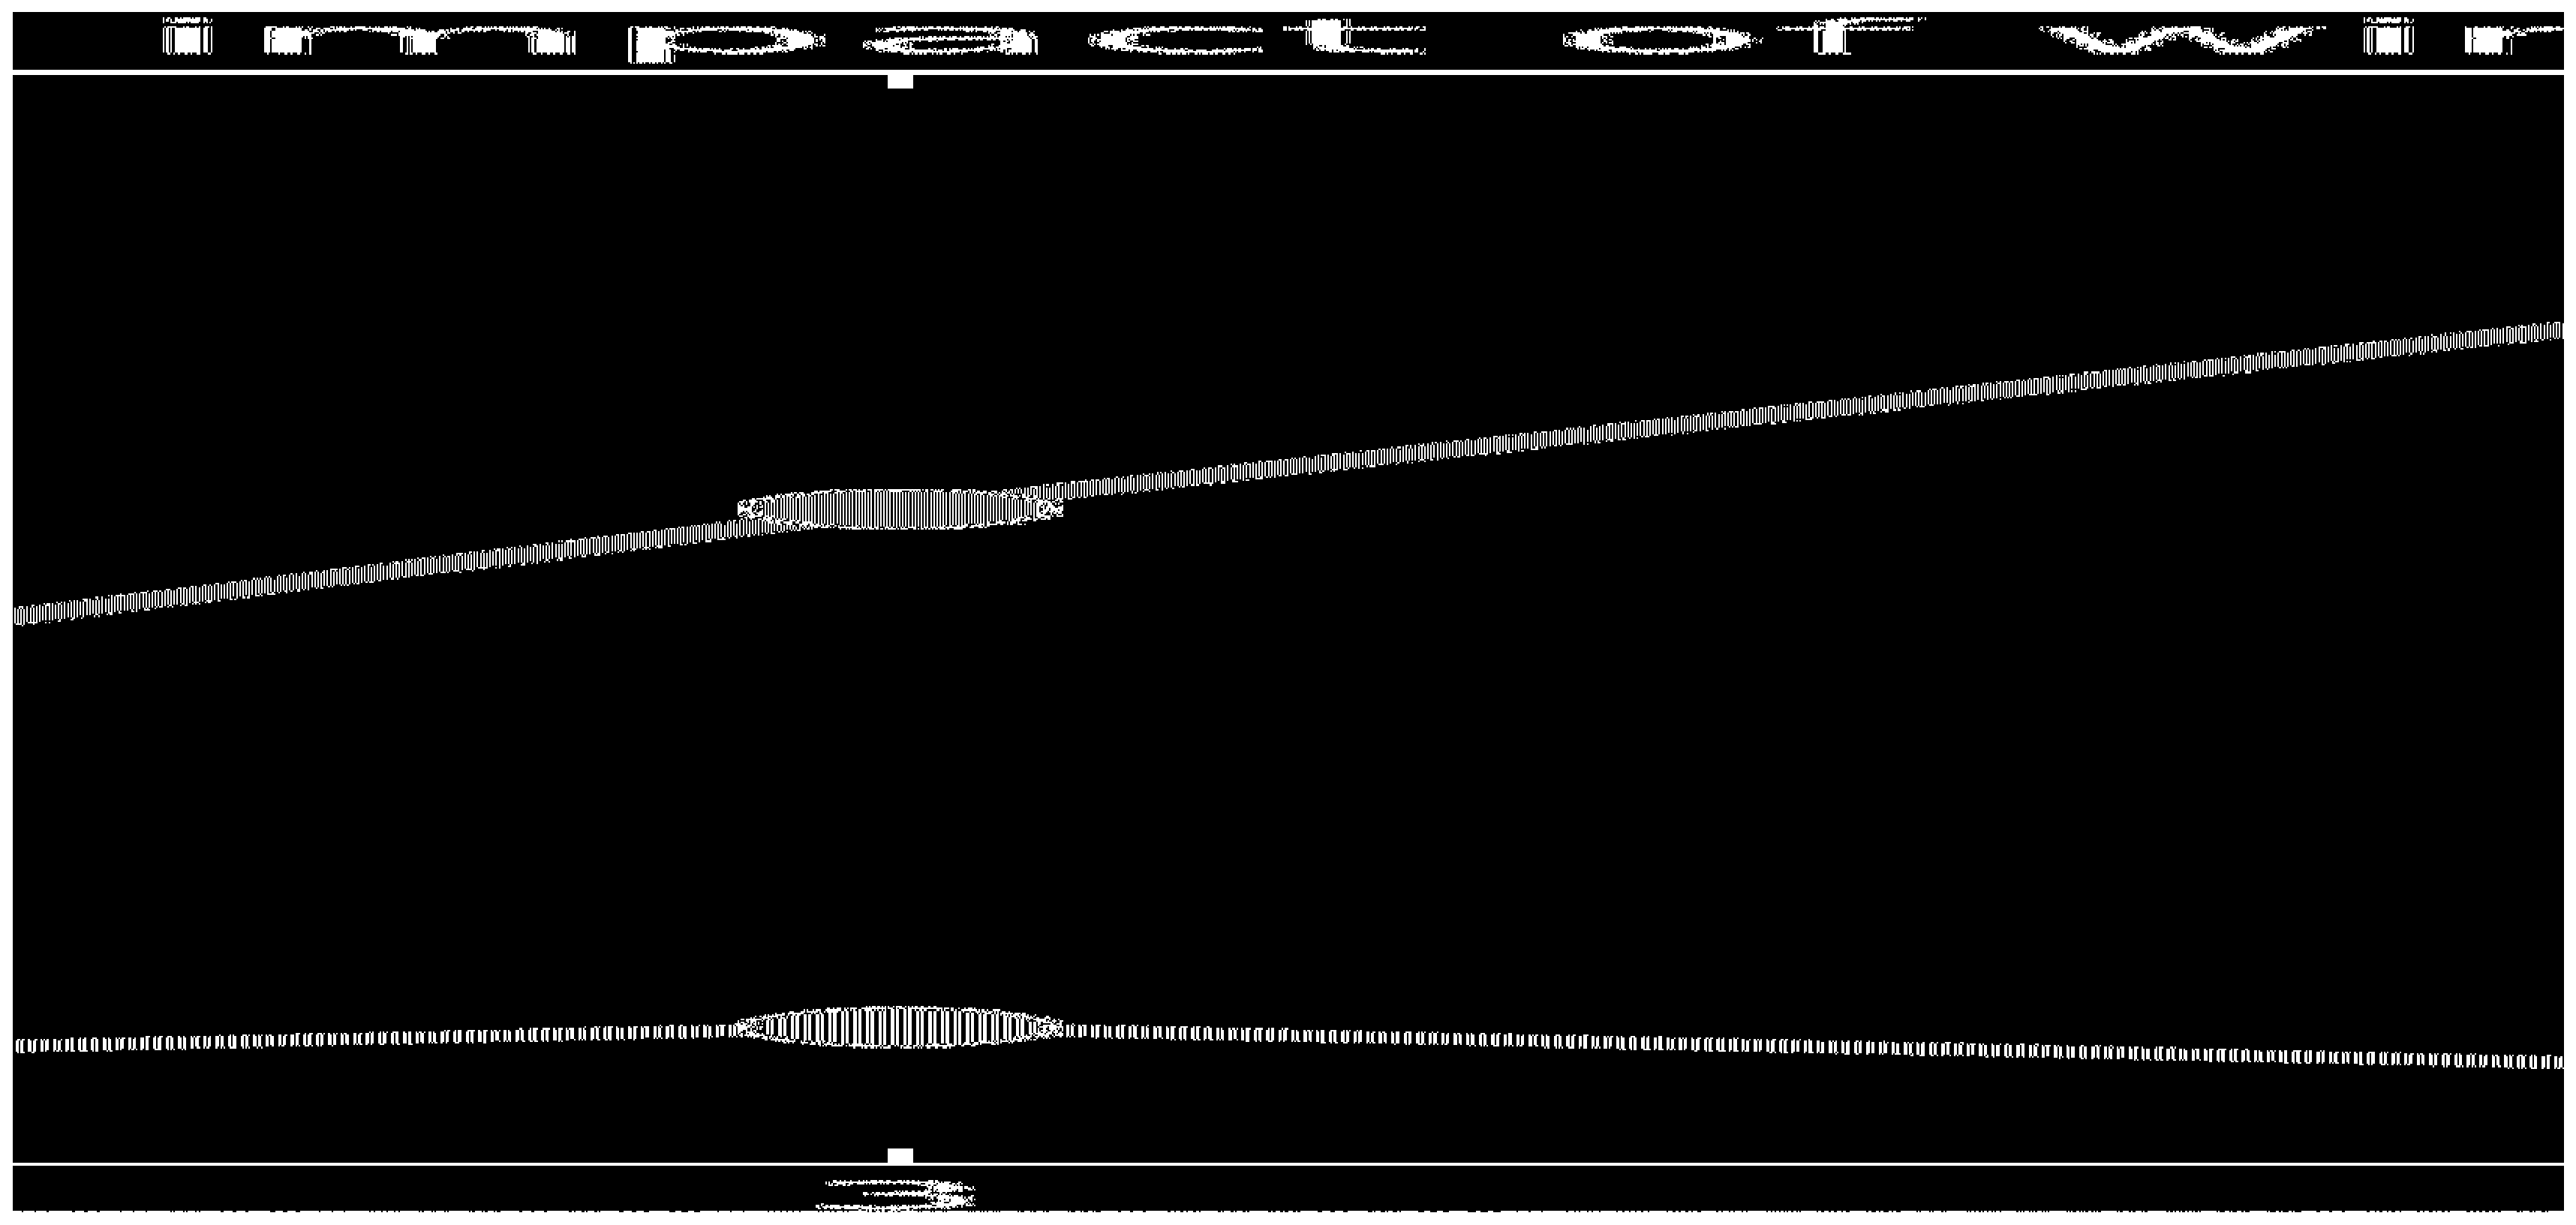
\includegraphics[width=69.09mm,height=32.51mm]{./CVPR2018_VideoSaliency_images/image017.eps.eps}
\end{center}
Figure 5. Sensitivities analysis on different window size settings.
\begin{center}
\begin{tabular}{|l|l|l|l|l|l|l|l|}
\hline
\multicolumn{1}{|l|}{DATASET}&	\multicolumn{1}{|l|}{LVO}&	\multicolumn{1}{|l|}{LVO+CRF}&	\multicolumn{1}{|l|}{FSEG}&	\multicolumn{1}{|l|}{LMP}&	\multicolumn{1}{|l|}{SFL}&	\multicolumn{1}{|l|}{OUS}&	\multicolumn{1}{|l|}{OUS+CRF}	\\
\hline
\multicolumn{1}{|l|}{DAVIS}&	\multicolumn{1}{|l|}{$70.9$}&	\multicolumn{1}{|l|}{ $75.9$}&	\multicolumn{1}{|l|}{ $70.7$}&	\multicolumn{1}{|l|}{ $70.0$}&	\multicolumn{1}{|l|}{ $67.4$}&	\multicolumn{1}{|l|}{ $73.0$}&	\multicolumn{1}{|l|}{ $77.1$}	\\
\hline
\multicolumn{1}{|l|}{FBMS}&	\multicolumn{1}{|l|}{$63.5$}&	\multicolumn{1}{|l|}{ $65.1$}&	\multicolumn{1}{|l|}{ $68.4$}&	\multicolumn{1}{|l|}{ $35.7$}&	\multicolumn{1}{|l|}{ $55.0$}&	\multicolumn{1}{|l|}{ $72.4$}&	\multicolumn{1}{|l|}{ $76.2$}	\\
\hline
\end{tabular}


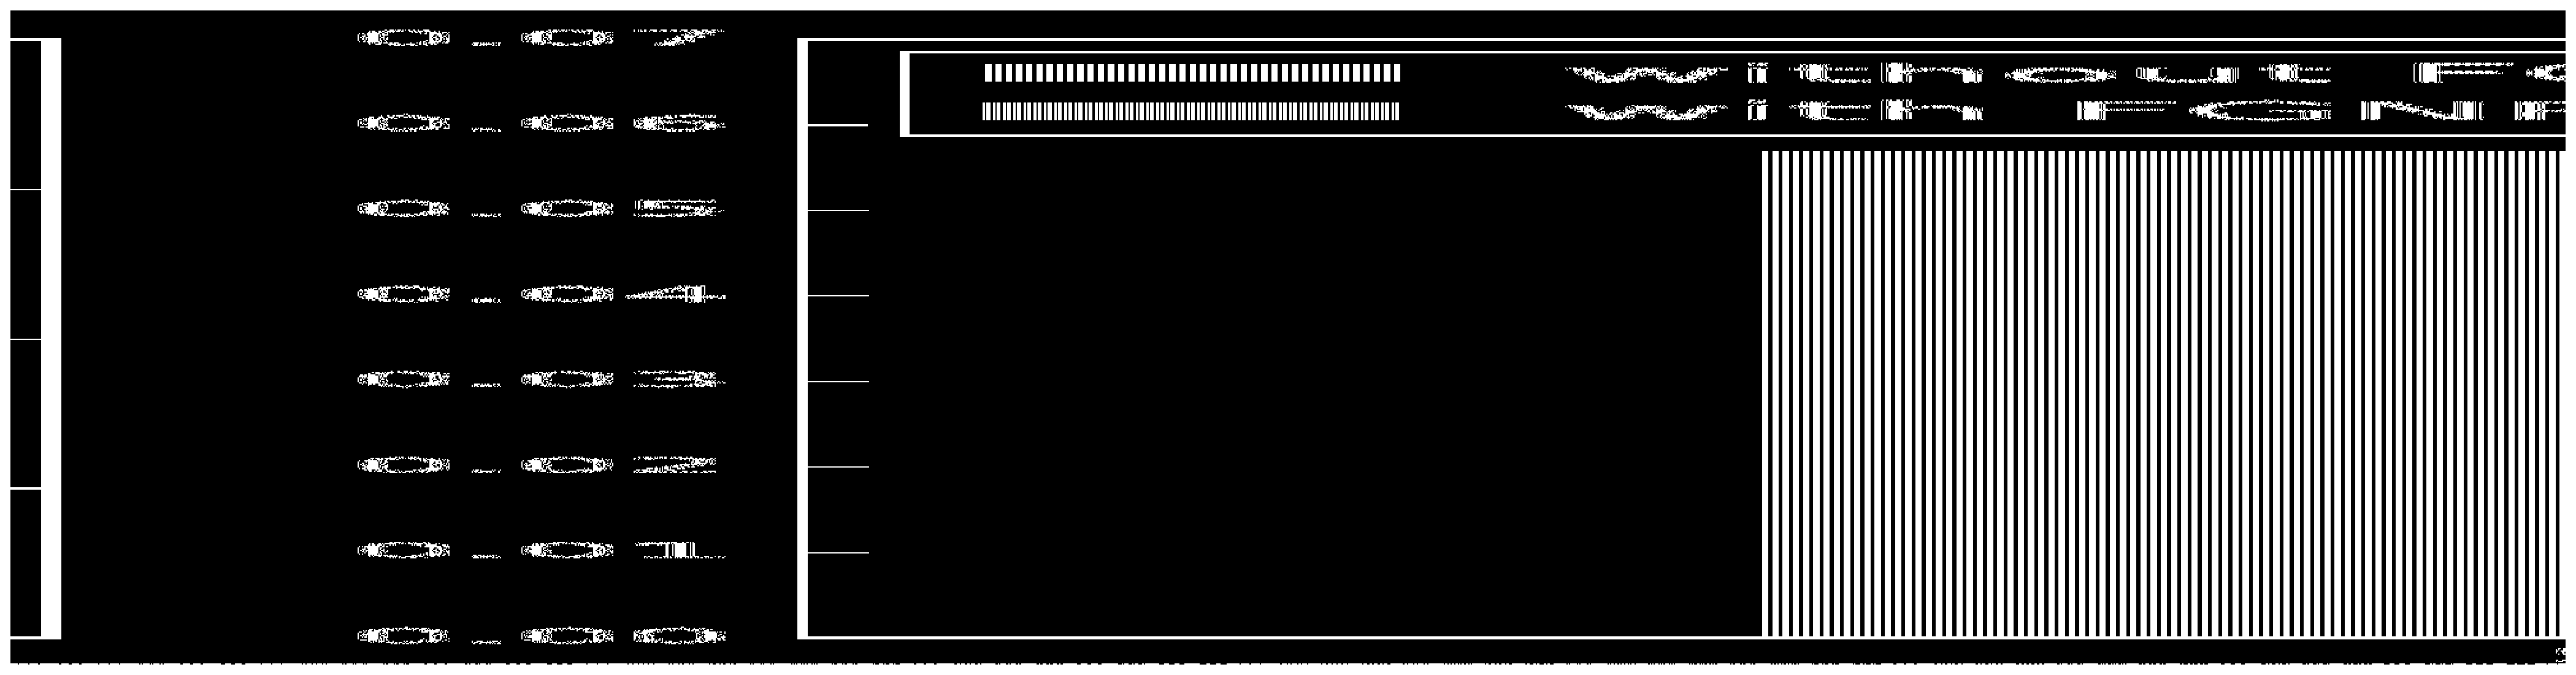
\includegraphics[width=84.67mm,height=21.67mm]{./CVPR2018_VideoSaliency_images/image018.eps.eps}
\end{center}
Figure 6. Sensitivities to host model selection.

layer as the host network is fully convolutional. We explore the effect of adding FGRNE to different levels of feature extraction on the performance of final results. We respec- tively experiment on adding feature encoding to the out- put feature map of Conv3 $-3$, Conv4 $-3$ and Conv5 $-3$ of the host DSS model. Experimental results shown that FGRNE is able to improve the temporal coherence on all scales of feature maps, which results in maxF value of 0:777, 0:789 and 0:798 respectively when choosing feature maps of Conv3 $-3$, Conv4-3 and Conv5 $-3$. Among them, incor- porating FGRNE with the feature extracted from Conv5 $-3$ results in the maximum performance gain, which increases the $\mathrm{F}$-measure by 2.97\% and decreases the MAE by 8.57\% w.r. $\mathrm{t}$ to its single-frame static version.

4.3.3 Sensitivities to Window Size Setting

Our proposed FGRNE learns to facilitate the temporal co- herence of the encoded feature by exploiting a window $k$ former frames. Limited by the memory of our workstation, $k$ can be set to amaximum of10. We have explored the impact of different settings of $k=\{1,2,3,5,8,10\}$ on the salient object detection performance. Results in Fig. 5 show that training with 5 and 8 former frames achieves very close accuracy, with $k=5$ performing slightly better. By default, we set $k=5$ during training and inference in our experi- ments.

4.3.4 Sensitivities to Host Model Selection

As described in Section 3, we adopt a FCN based static saliency detector as the host model for our FGRNE. To demonstrate that our proposed method is widely applica- ble to any FCN based host network model, we apply to in- corporate our FGRNE in two other recently published FCN based salient object detection methods, including DCL $[^{:}24_{-}0$]

and MSRNet $[1_{\ovalbox{\tt\small REJECT}}8_{\ovalbox{\tt\small REJECT}}]$. For the latter, due to the limitation of machine memory, we only experiment on its single scale version, i.e. SSRNet. As shown in Fig. 6, experimental evaluation on both $\mathrm{F}$-measure and MAE have shown that our FGRNE can be trained to effectively enhance the spatio- temporal coherence of the feature representation, which greatly boost the performance of video salient object de- tection.

Table 3. Performance comparison on unsupervised video object segmentation in terms of mean $\mathrm{I}\mathrm{o}\mathrm{U}$

5. Comparison with Unsupervised Video Ob- ject Segmentation Methods

The problem setting of video salient object detection is very similar to that of unsupervised video object segmen- tation, except that its goal is to calculate a saliency proba- bility value for each pixel instead of a binary classification. To make a fair comparison with the state-of-the-art unsu- pervised video object segmentation methods, we incorpo- rate our FGRNE with a static ResNet-101 based pixel-wise binary classification model with feature extracted from the final output feature map of Conv5-X. We evaluate our pro- posed method on both the DAVIS and FBMS datasets in terms of mean $\mathrm{I}\mathrm{o}\mathrm{U}$ and make a comparison with some state- of-the-art methods. As shown in Table 3, our proposed method outperforms LVO $[^{:}2_{\nu}^{\fbox{$\mathrm{Error}::0\mathrm{x}0000$}}(:\dot{9}$], the previous state of the art, by 2.96\% and 14.0\% on the $\mathrm{I}\mathrm{o}\mathrm{U}$ measure respectively on DAVIS and FBMS. Noted that as described in $[2^{(:}\fbox{$\mathrm{Error}::0\mathrm{x}0000$}.9]$, the mIoU value of 75.9\% reported on the leaderboard of DAVIS includes CRF as post-processing, the result of LVO without CRF is 70.9 as reported in their paper. For fair comparison, we also report our mIoU results with and without CRF in the table. As can be seen, our proposed method with CRF also greatly outperforms LVO by 1.6\% and 16.90\% respec- tively on DAVIS and FBMS.

6. Conclusion

In this paper, we have presented an accurate and end- to-end framework for video salient object detection. Our proposed flow guided recurrent encoder aims at improving the temporal coherence of the deep feature representation. It can be considered as a universal framework to extend any FCN based static saliency detector to video salient ob- ject detection, and can easily benefit from the future im- provement of image based salient object detection methods. Moreover, as we focus on the learning an enhanced feature encoding, it can be easily extended to other applications of video analysis and it is worth exploring in the future.

References

[1] R. Achanta, S. Hemami, F Estrada, and S. Susstrunk. Frequency-tuned salient region detection. In {\it CVPR}, pages 15971604. IEEE, 2009. 5

[2] T Brox and J. Malik. Object segmentation by long term analysis of point trajectories. {\it ECCV}, pages 282295, 2010. 5

[3] C. Chen, S. Li, Y Wang, H. Qin, and A. Hao. Video saliency detection via spatial-temporal fusion and low-rank coherency diffusion. {\it TIP}, $26(7):3156-3170$, 2017. 1, 2, 3

[4] T Chen, M. Li, Y Li, M. Lin, N. Wang, M. Wang, T Xiao, B. Xu, C. Zhang, and Z. Zhang. Mxnet: A flexible and effi- cient machine learning library for heterogeneous distributed systems. {\it arXiv preprint arXiv}:{\it 1512.01274}, 2015. 5

[5] M.-M. Cheng, N. J. Mitra, X. Huang, P. H. Torr, and S.-M. Hu. Global contrast based salient region detection. {\it TPAMI}, $37(3):569-582$, 2015. 2

[6] Y Fang, Z. Wang, W Lin, and Z. Fang. Video saliency in- corporating spatiotemporal cues and uncertainty weighting. {\it TIP}, $23(9):3910-3921$, 2014. 3

[7] P Fischer, A. Dosovitskiy, E. Ilg, P H"\""{a}"usser, C. Haz{\imath}rbas, V Golkov, P. van der Smagt, D. Cremers, and T Brox. Flownet: Learning optical flow with convolutional networks. {\it arXiv preprint arXiv}:{\it 1504.06852}, 2015. 2, 3, 4

[8] D. Gao and N. Vasconcelos. Bottom-up saliency is a dis- criminant process. In {\it ICCV}, pages 16. IEEE, 2007. 2

[9] C. Guo, Q. Ma, and L. Zhang. Spatio-temporal saliency detection using phase spectrum of quaternion fourier trans- form. In {\it CVPR}, pages 18. IEEE, 2008. 3

[10] Q. Hou, M.-M. Cheng, X.-W. Hu, A. Borji, Z. Tu, and P Torr. Deeply supervised salient object detection with short con- nections. {\it arXiv preprint arXiv}:{\it 1611.04849}, 2016. 1, 2, 3, 5, 6

[11] E. Ilg, N. Mayer, T. Saikia, M. Keuper, A. Dosovitskiy, and T Brox. Flownet 2.0: Evolution of optical flow estimation with deep networks. {\it arXiv preprint arXiv}:{\it 1612.01925}, 2016. 3

[12] L. Itti. Automatic foveation for video compression using a neurobiological model of visual attention. {\it TIP}, 13(10): 1304- 1318, 2004. 1

[13] L. Itti, C. Koch, and E. Niebur. A model of saliency-based vi- sual attention for rapid scene analysis. {\it TPAMI}, 20(11): 1254- 1259, 1998. 1

[14] Y Jia and M. Han. Category-independent object-level saliency detection. In {\it ICCV}, pages 17611768, 2013. 2

[15] H. Jiang, J. Wang, Z. Yuan, Y Wu, N. Zheng, and S. Li. Salient object detection: A discriminative regional feature integration approach. In {\it CVPR}, pages 20832090, 2013. 2

[16] T-N. Le and A. Sugimoto. Video salient object detec- tion using spatiotemporal deep features. {\it arXiv preprint arXiv}:{\it l708.01447}, 2017. 2, 3

[17] G. Lee, Y.-W. Tai, and J. Kim. Deep saliency with encoded low level distance map and high level features. In {\it CVPR}, pages 660668, 2016. 2

[18] G. Li, Y Xie, L. Lin, and Y Yu. Instance-level salient object segmentation. {\it arXiv preprint arXiv}:{\it l704.03604}, 2017. 1, 2, 3, 8

[19] G. Li and Y Yu. Visual saliency based on multiscale deep features. In {\it CVPR}, pages 54555463, 2015. 2

[20] G. Li and Y Yu. Deep contrast learning for salient object detection. In {\it CVPR}, pages 478487, 2016. 1, 2, 3, 6, 8

[21] G. Li and Y Yu. Visual saliency detection based on multi- scale deep cnn features. {\it TIP}, $25(11):5012-5024$, 2016. 1

[22] Y Li, X. Hou, C. Koch, J. M. Rehg, and A. L. Yuille. The secrets of salient object segmentation. In {\it CVPR}, pages 280- 287, 2014. 2

[23] N. Liu and J. Han. Dhsnet: Deep hierarchical saliency net- work for salient object detection. In {\it CVPR}, pages 678686, 2016. 3, 6

[24] V Mahadevan and N. Vasconcelos. Spatiotemporal saliency in dynamic scenes. {\it TPAMI}, 32(1): 171-177, 2010. 3

[25] P Ochs, J. Malik, and T. Brox. Segmentation of moving objects by long term video analysis. {\it TPAMI}, 36(6): 1187- 1200, 2014. 5

[26] F Perazzi, P Krahenbuhl, Y Pritch, and A. Hornung. Saliency filters: Contrast based filtering for salient region detection. In {\it CVPR}, 2012. 5

[27] F Perazzi, J. Pont-Tuset, B. McWilliams, L. Van Gool, M. Gross, and A. Sorkine-Hornung. A benchmark dataset and evaluation methodology for video object segmentation. In {\it CVPR}, pages 724732, 2016. 5

[28] A. Ranjan and M. J. Black. Optical flow estimation using a spatial pyramid network. {\it arXiv preprint arXiv}:{\it 1611.00850}, 2016. 3

[29] P Tokmakov, K. Alahari, and C. Schmid. Learning video object segmentation with visual memory. {\it arXiv preprint arXiv}:{\it l704.05737}, 2017. 3, 8

[30] D. Tsai, M. Flagg, A. Nakazawa, and J. M. Rehg. Motion coherent tracking using multi-label mrf optimization. {\it IJCV}, $100(2):190-202$, 2012. 5

[31] W.-C. Tu, S. He, Q. Yang, and S.-Y Chien. Real-time salient object detection with a minimum spanning tree. In {\it CVPR}, pages 23342342, 2016. 6

[32] L. Wang, H. Lu, X. Ruan, and M.-H. Yang. Deep networks for saliency detection via local estimation and global search. In {\it CVPR}, pages 31833192, 2015. 2

[33] L. Wang, L. Wang, H. Lu, P Zhang, and X. Ruan. Saliency detection with recurrent fully convolutional networks. In {\it ECCV}, pages 825841. Springer, 2016. 2, 3, 6

[34] W Wang, J. Shen, and F. Porikli. Saliency-aware geodesic video object segmentation. In {\it CVPR}, pages 33953402, 2015. 6

[35] W Wang, J. Shen, and L. Shao. Consistent video saliency using local gradient flow optimization and global refinement. {\it TIP}, $24(11):4185-4196$, 2015. 1, 2, 3, 6

[36] W Wang, J. Shen, and L. Shao. Video salient object de- tection via fully convolutional networks. {\it TIP}, $27(1):38-49,$ 2018. 1, 2, 5, 6

[37] Y Wei, X. Liang, Y Chen, X. Shen, M.-M. Cheng, J. Feng, Y Zhao, and S. Yan. Stc: A simple to complex frame- work for weakly-supervised semantic segmentation. {\it TPAMI}, $39(11):2314-2320$, 2017. 1

[38] H. Wu, G. Li, and X. Luo. Weighted attentional blocks for probabilistic object tracking. {\it The Visual Computer}, $30(2):229-243$, 2014. 1

[39] S. Xingjian, Z. Chen, H. Wang, D.-Y Yeung, W.-K. Wong, and W.-c. Woo. Convolutional lstm network: A machine learning approach for precipitation nowcasting. In {\it NIPS}, pages 802810, 2015. 4

[40] J. Yang and M.-H. Yang. Top-down visual saliency viajoint crf and dictionary learning. In {\it CVPR}, pages 22962303. IEEE, 2012. 2

[41] J. Zhang, S. Sclaroff, Z. Lin, X. Shen, B. Price, and R. Mech. Minimum barrier salient object detection at 80 fps. In {\it ICCV}, pages 14041412, 2015. 6

[42] R. Zhao, W Ouyang, H. Li, and X. Wang. Saliency detection by multi-context deep learning. In {\it CVPR}, pages 12651274, 2015. 2

[43] R. Zhao, W Ouyang, and X. Wang. Unsupervised salience learning for person re-identification. In {\it CVPR}, pages 3586- 3593, 2013. 1

[44] X. Zhu, Y Wang, J. Dai, L. Yuan, and Y Wei. Flow-guided feature aggregation for video object detection. {\it arXiv preprint arXiv}:{\it l 703.10025}, 2017. 3

[45] X. Zhu, Y Xiong, J. Dai, L. Yuan, and Y Wei. Deep feature flow for video recognition. {\it arXiv preprint arXiv}:{\it 1611.07715}, 2016. 3, 4
\end{document}
